% ============================================================
% Project 2 (PDE BVP) --- LaTeX Report
% Numerical Valuation of Perpetual American Put Options via LCP
% Compile: pdflatex report.tex  (twice to resolve the TOC and citations)
% ============================================================

\documentclass[11pt,a4paper]{article}

\usepackage[utf8]{inputenc}
\usepackage[T1]{fontenc}
\usepackage{amsmath, amssymb, amsthm}
\usepackage{geometry}
\geometry{a4paper, margin=2.5cm}
\usepackage{graphicx}
\graphicspath{{./}}
\usepackage{booktabs}
\usepackage{array}
\usepackage{longtable}
\usepackage{listings}
\usepackage{xcolor}
\usepackage{hyperref}
\usepackage{enumitem}
\usepackage{float}
\usepackage{caption}
\usepackage{subcaption}
\usepackage{bm}
\usepackage{algorithm}
\usepackage{algpseudocode}
\usepackage{mdframed}

% --- colors ---
\definecolor{lecture}{RGB}{70,130,180}
\definecolor{seminar}{RGB}{205,92,92}
\definecolor{formbg}{RGB}{250,250,245}
\definecolor{formframe}{RGB}{180,170,140}

% --- code listing style (Python) ---
\lstset{
    language=Python,
    basicstyle=\ttfamily\scriptsize,
    keywordstyle=\color{blue}\bfseries,
    commentstyle=\color{green!40!black},
    stringstyle=\color{red!70!black},
    numbers=left,
    numberstyle=\tiny\color{gray},
    frame=single,
    breaklines=true,
    showstringspaces=false,
    tabsize=4,
    captionpos=b,
}

% --- theorem-like environments (course-level set) ---
\newtheorem{theorem}{Theorem}[section]
\newtheorem{lemma}[theorem]{Lemma}
\newtheorem{proposition}[theorem]{Proposition}
\newtheorem{corollary}[theorem]{Corollary}
\theoremstyle{definition}
\newtheorem{definition}[theorem]{Definition}
\newtheorem{assumption}[theorem]{Assumption}
\newtheorem{example}[theorem]{Example}
\theoremstyle{remark}
\newtheorem{remark}[theorem]{Remark}

% --- algorithm style ---
\algrenewcommand{\algorithmicrequire}{\textbf{Input:}}
\algrenewcommand{\algorithmicensure}{\textbf{Output:}}
\algrenewcommand{\algorithmiccomment}[1]{\hfill\textcolor{gray}{\# #1}}

% --- form box (for appendices) ---
\newmdenv[
    backgroundcolor=formbg,
    linecolor=formframe,
    linewidth=0.8pt,
    roundcorner=3pt,
    innermargin=5pt,
    outermargin=5pt,
    innertopmargin=8pt,
    innerbottommargin=8pt
]{formbox}

\title{\textbf{Numerical Valuation of Perpetual American Put Options via LCP}\\[2mm]
\large Project 2 (PDE BVP) Report}
\author{
    \small Team number: Group L\\
    \small Yuhan Cheng \quad Student ID: 2685836\\
    \small Yijian Huang \quad Student ID: 2685589\\
    \small Department of Applied Mathematics
}
\date{\today}

\begin{document}
\maketitle

\begin{abstract}
\noindent
This report treats the perpetual American put as an elliptic obstacle problem
whose solution must satisfy a linear complementarity problem (LCP). The early
exercise boundary is not prescribed in advance; it is recovered as the
interface between the exercise and continuation regions. The spatial operator
is discretised on a uniform grid by exponential fitting in the
Scharfetter--Gummel form. The fitted weights are positive, the two
off-diagonal entries are non-positive, and the row sum is strictly positive,
so the discrete operator is an M-matrix at every cell P\'eclet number,
including the degenerate region near $S=0$. This structure yields a discrete
maximum principle and a unique obstacle solution. The LCP is solved by policy
iteration with sparse direct linear solves. For constant volatility and
$q=0$, the production $N=2400$ contact bracket is $[71,72]$ and contains the
exact free boundary $S^*=71.4286$. Because a production contact bracket is
phase sensitive, the stencil order is measured separately on a
boundary-aligned validation grid: the errors range from
$1.073\times10^{-2}$ to $1.682\times10^{-4}$, with successive ratios
$3.990$, $4.001$, and $3.997$. For local volatility and $q=0.02$, an
independent DOP853 shooting solution of the free-boundary ODE gives
$S^*=69.1664$ and $V(100)=16.2055$. The $N=2400$ production estimate
$S_h^*=69.1688$ lies in $[69,70]$, whereas the coarse $N=1200$ contact
bracket $[70,72]$ misses the reference; this coarse-grid localisation error
is reported rather than treated as convergence evidence. The aligned
finite-difference sequence has ratios $3.980$, $4.000$, and $3.999$. At
$S=100$ the pure finite-domain truncation is $5.578\times10^{-3}$, the
$N=2400$ production total error is $4.055\times10^{-3}$ after partial
error cancellation, and the far-edge truncation is
$4.833\times10^{-1}$. At the benchmark mesh,
policy iteration requires 301 iterations and $0.045$~s, whereas projected
successive over-relaxation needs 96{,}600 iterations and $20.635$~s. The
measured $4.6\times10^2$ wall-time ratio, together with the 321-fold
iteration reduction, places the acceleration in the several-hundred-fold
range. On a nonuniform grid the same fitted
construction reduces the maximum value error by a factor of $2.255$ at
$N=2400$ when nodes are clustered around the free boundary, while an
asymptotic Robin closure reduces the far-field error by up to three orders
of magnitude. A discrete adjoint formulation provides the sensitivities of
$V(100)$ to $\sigma$, $r$, and $q$ with one extra linear solve, matching
direct finite differences to $2\times10^{-9}$ and exact derivatives to
$0.31\%$. A controlled two-dimensional spread-put extension with $\rho=0$
retains the five-point M-matrix structure; its pricing-window error decreases
from $4.070\times10^{-2}$ to $1.611\times10^{-2}$ between $N=80$ and $N=160$,
and its value at $(100,50)$ changes by only $9.71\times10^{-4}$ when the domain
is enlarged from $L=300$ to $L=400$. The remaining limitations are the fully
front-fitted treatment of the free-boundary kink, the finite-domain
truncation of the production Dirichlet solve, and the restriction of the 2D
experiment to zero correlation with approximate high-price closures.
\end{abstract}

\noindent\raggedright\textbf{Keywords:} perpetual American put, linear complementarity
 problem, exponential fitting, Scharfetter--Gummel, policy iteration, free
 boundary, local volatility, adaptive mesh, Robin boundary, adjoint
 sensitivity, M-matrix

\tableofcontents
\newpage

% ============================================================
\section{Introduction and Motivation}
% ============================================================

\subsection{Problem Background}
An American put gives its holder the right, but not the obligation, to sell
one unit of an underlying asset at strike $K$ at any time before expiry. The
value is therefore an optimal stopping value: at every state the holder
compares the payoff obtained by immediate exercise with the expected
discounted value obtained by continuing to hold the contract. The standard
risk-neutral treatment of this decision is developed in
\cite{ref1,ref2}. In the perpetual limit the remaining maturity tends to
infinity, the time derivative disappears, and the valuation reduces to an
elliptic boundary-value problem posed on the positive half-line.

The elliptic reduction retains the central difficulty of the American-option
problem: the set on which exercise is optimal is not known a priori. It is
separated from the continuation set by a free boundary $S^*$. On the exercise
side the value equals the put payoff; on the continuation side it satisfies
the homogeneous Black--Scholes equation; at the interface the two branches
meet with continuous value and derivative. A method that solves only the
partial differential equation must first locate $S^*$ and then impose the
matching conditions. An obstacle formulation avoids this two-stage procedure.
It enforces the differential inequality and the payoff constraint
simultaneously, and it treats the exercise region as part of the unknown
solution.

This formulation is attractive for three reasons. First, the shape of the
domain is fixed, so no moving-mesh or front-fixing transformation is required.
Second, the problem becomes a finite-dimensional linear complementarity
problem (LCP) after discretisation. Third, the discrete LCP inherits the
monotonicity of the differential operator when the stencil is chosen
correctly, which gives both a comparison principle and a stable active-set
algorithm. The finite-difference and obstacle formulations used here follow
the classical treatment in \cite{ref2}; recent high-order and LCP methods for
free-boundary options are represented by \cite{ref3,ref9}.

The numerical difficulty near $S=0$ deserves separate emphasis. The diffusion
coefficient in the Black--Scholes operator is proportional to $S^2$, while
the drift coefficient is proportional to $S$. Their ratio, expressed as a
cell P\'eclet number, does not vanish as the mesh is refined. A central
difference of the drift term can consequently produce a positive
off-diagonal entry and destroy the M-matrix property. The resulting
oscillation is not a cosmetic artefact: it violates the discrete maximum
principle and can contaminate the computed exercise boundary. Exponential
fitting removes this failure by adapting the difference weights to the local
ratio of drift to diffusion.

\subsection{Mathematical Model}
Let $S\in[0,S_{\max}]$ denote the stock price, $r>0$ the risk-free rate,
$q\ge0$ the dividend yield, and $\sigma(S)>0$ the local volatility. The put
payoff is
\begin{equation}
    \psi(S)=\max(K-S,0).
    \label{eq:payoff}
\end{equation}
Under the risk-neutral measure the stock evolves as
\begin{equation}
    \mathrm{d}S_t=(r-q)S_t\,\mathrm{d}t+\sigma(S_t)S_t\,\mathrm{d}W_t,
    \label{eq:sde}
\end{equation}
and the infinitesimal generator of the discounted value is
\begin{equation}
    \mathcal{L}V
    =\frac12\sigma(S)^2S^2V''+(r-q)SV'-rV.
    \label{eq:operator}
\end{equation}
For the perpetual put, the value is independent of calendar time and satisfies
the complementarity conditions
\begin{equation}
    V\ge\psi,
    \qquad
    -\mathcal{L}V\ge0,
    \qquad
    (V-\psi)(-\mathcal{L}V)=0,
    \label{eq:complementarity}
\end{equation}
or, in compact form,
\begin{equation}
    \min\left(-\mathcal{L}V,\;V-\psi\right)=0,
    \qquad 0<S<S_{\max}.
    \label{eq:lcp}
\end{equation}
The boundary conditions are
\begin{equation}
    V(0)=K,
    \qquad
    V(S_{\max})=0.
    \label{eq:boundaries}
\end{equation}
The left condition is exact: at zero the put is certain to be exercised. The
right condition is a truncation of the positive half-line and is therefore a
numerical boundary condition. Its effect is quantified separately in
Section~\ref{sec:localvol}.

Two parameter sets are used. The constant-volatility verification problem has
\begin{equation}
    K=100,
    \qquad r=0.05,
    \qquad q=0,
    \qquad \sigma=0.20,
    \qquad S_{\max}=2400.
    \label{eq:parameters-stage1}
\end{equation}
The local-volatility experiment keeps $K$, $r$, and $S_{\max}$ fixed, sets
$q=0.02$, and uses
\begin{equation}
    \sigma(S)=0.20\left[
    1+0.35\tanh\left(\frac{\log(S/K)}{0.40}\right)\right].
    \label{eq:localvol}
\end{equation}
This profile is smooth and bounded away from zero. It is below $0.20$ for
$S<K$ and above $0.20$ for $S>K$, so it changes both the early-exercise
premium and the far-field decay.

\subsection{Free-Boundary Characterisation and Analytic Benchmark}
For a perpetual put the exercise region is an interval $[0,S^*]$ and the
continuation region is $(S^*,\infty)$. On the exercise side,
$V(S)=K-S$ and hence
\begin{equation}
    -\mathcal{L}\psi
    =rK-qS.
    \label{eq:exercise-operator}
\end{equation}
On the continuation side, $V$ solves $-\mathcal{L}V=0$. At the free boundary
the value and its first derivative are continuous:
\begin{equation}
    V(S^*)=K-S^*,
    \qquad
    V'(S^*)=-1.
    \label{eq:smooth-pasting}
\end{equation}
These two conditions replace an unknown boundary location by a local
matching condition and are the classical form of the smooth-pasting
principle.

For constant coefficients, substitution of $V(S)=S^\lambda$ into
$-\mathcal{L}V=0$ gives the indicial equation
\begin{equation}
    \frac12\sigma^2\lambda(\lambda-1)
    +\left[(r-q)-\frac12\sigma^2\right]\lambda-r=0.
    \label{eq:indicial}
\end{equation}
Its roots are
\begin{equation}
    \lambda_{\pm}
    =\frac12-\frac{r-q}{\sigma^2}
    \pm\sqrt{\left(\frac{r-q}{\sigma^2}-\frac12\right)^2
    +\frac{2r}{\sigma^2}}.
    \label{eq:roots}
\end{equation}
The decaying branch is $\lambda_-$; the other root grows and is inadmissible
for a put. Smooth pasting gives
\begin{equation}
    S^*=\frac{\lambda_-K}{\lambda_--1}.
    \label{eq:exactboundary}
\end{equation}
For \eqref{eq:parameters-stage1}, $\lambda_-=-2.5$ and
\begin{equation}
    S^*=71.4285714286,
    \qquad
    V(S)=(K-S^*)\left(\frac{S}{S^*}\right)^{-2.5},
    \quad S>S^*.
    \label{eq:exactvalue}
\end{equation}
In particular, $V(100)=12.3200328678$. This closed form is used only for
verification; the production solver does not impose the analytic tail at the
truncation boundary.

The dividend yield moves the boundary in the opposite direction to the
local-volatility level. With $q=0.02$ and constant $\sigma=0.20$, the same
formula gives $S^*=64.9219$. Around the local-volatility boundary the profile
\eqref{eq:localvol} is approximately $0.149$, which lowers the value of
continuation and pushes the boundary upward relative to the constant
$q=0.02$ case. The computed value $S_h^*=69.17$ is the net result of these
two effects.

\subsection{Overview of the Report}
Section~\ref{sec:discretisation} constructs the exponentially fitted
 operator, proves its M-matrix property, analyses consistency and stability,
 and treats the Dirichlet and free-boundary conditions; it also develops a
 nonuniform fitted operator, an asymptotic Robin closure, multi-point
 boundary extraction, and discrete adjoint sensitivities. Section
\ref{sec:implementation} describes the policy-iteration algorithm and its
implementation. Section~\ref{sec:experiments} contains the convergence study,
the two-solver comparison and a tolerance sweep that separate algebraic from
discretisation error, the local-volatility and domain-truncation experiments,
the adaptive-grid and Robin-closure studies, the Greeks, adjoint sensitivities,
and the limitations of the approach. Section~\ref{sec:spread2d} adds a controlled two-dimensional
 spread-put LCP as a scaling and structure test. Section~\ref{sec:conclusions}
 summarises the conclusions.
Appendices~\ref{app:ai} and~\ref{app:ics} contain the AI transparency log and
the individual contribution statements.

\newpage
% ============================================================
\section{Discretisation and Analysis}
\label{sec:discretisation}
% ============================================================

\subsection{Discrete Scheme}
The computational domain is divided by the uniform grid
\begin{equation}
    S_i=ih,
    \qquad
    h=\frac{S_{\max}}{N},
    \qquad
    i=0,1,\ldots,N.
    \label{eq:grid}
\end{equation}
At the interior nodes define
\begin{equation}
    a_i=\frac12\sigma(S_i)^2S_i^2,
    \qquad
    b_i=(r-q)S_i,
    \qquad
    \operatorname{Pe}_i=\frac{b_ih}{a_i}.
    \label{eq:coefficients}
\end{equation}
The quantity $\operatorname{Pe}_i$ is the cell P\'eclet number. It measures
the relative importance of drift and diffusion on the cell adjacent to
$S_i$. It is not assumed to be small. For constant coefficients, at the first
interior node,
\begin{equation}
    \operatorname{Pe}_1=\frac{2(r-q)}{\sigma^2},
    \label{eq:first-peclet}
\end{equation}
independently of $h$. With the Stage~1 parameters this value is $2.5$, which
is already beyond the central-difference stability limit. Thus the
near-origin degeneracy does not disappear under mesh refinement.

For comparison, central differencing of the drift term gives the
coefficients
\begin{equation}
    \ell_i^{\mathrm{CD}}=-\frac{a_i}{h^2}+\frac{b_i}{2h},
    \qquad
    u_i^{\mathrm{CD}}=-\frac{a_i}{h^2}-\frac{b_i}{2h}.
    \label{eq:central}
\end{equation}
When $\operatorname{Pe}_i>2$ the lower off-diagonal becomes positive, and
when $\operatorname{Pe}_i<-2$ the upper off-diagonal becomes positive. A
single positive off-diagonal is enough to violate the sign condition required
of an M-matrix.

\begin{figure}[H]
\centering
\begin{subfigure}{0.48\textwidth}
\centering
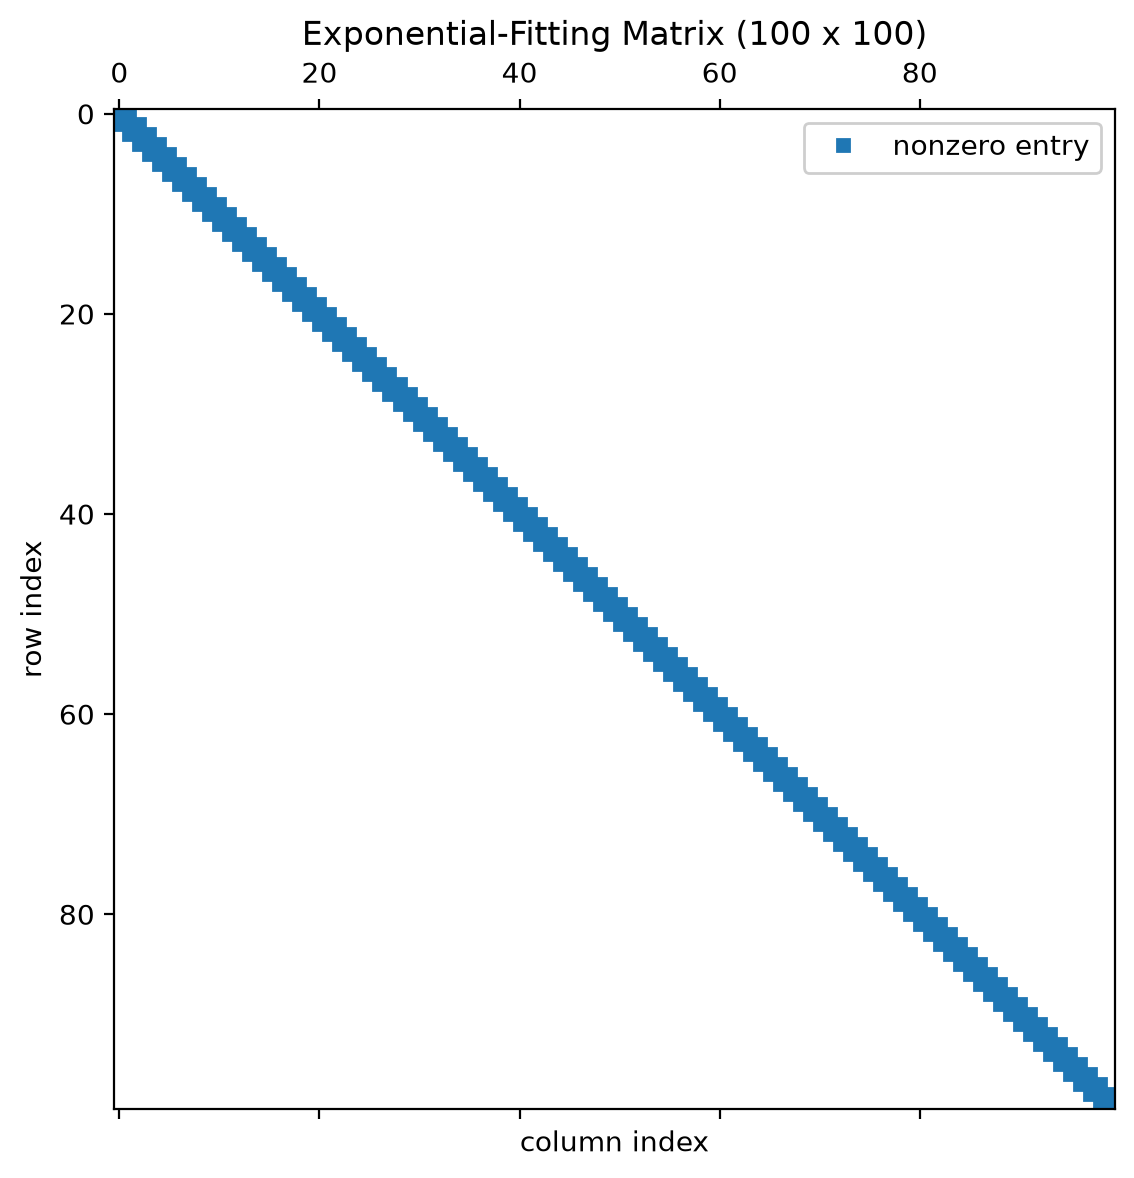
\includegraphics[width=\linewidth]{matrix_spy_fitted.png}
\caption{Exponential Fitting}
\label{fig:matrix_spy_fitted}
\end{subfigure}
\hfill
\begin{subfigure}{0.48\textwidth}
\centering
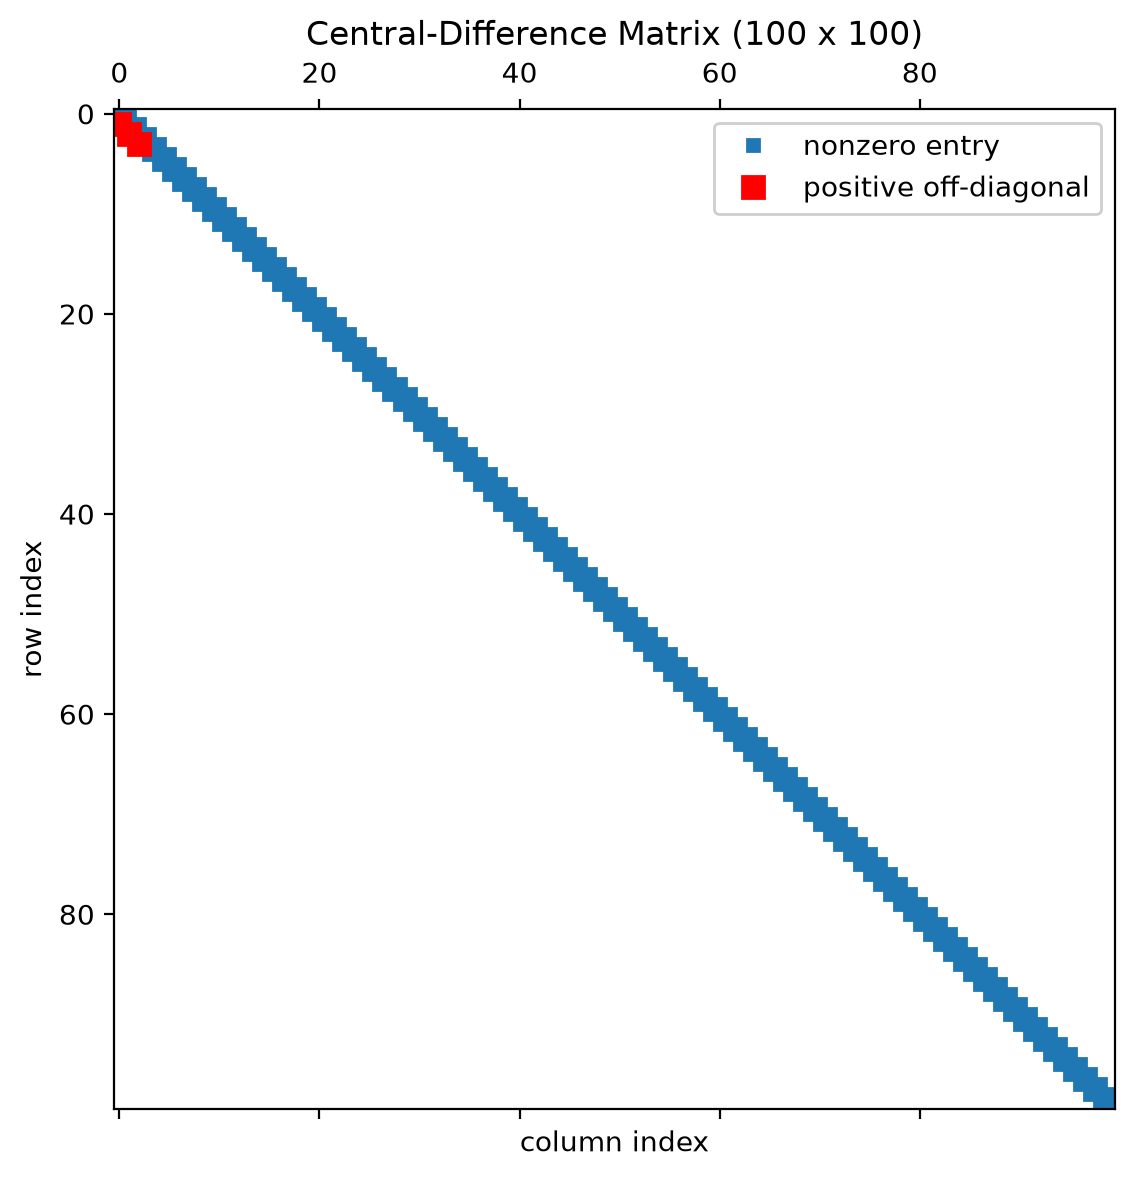
\includegraphics[width=\linewidth]{matrix_spy_central.png}
\caption{Central Differencing}
\label{fig:matrix_spy_central}
\end{subfigure}
\caption{Spy plots of the $100\times100$ fitted and central-difference
matrices. Near $S=0$, central differencing produces positive off-diagonal
entries (red), destroying the M-matrix property. The exponentially fitted
matrix has non-positive off-diagonal entries throughout.}
\label{fig:matrix_spy}
\end{figure}

Figure~\ref{fig:matrix_spy} shows this sign change directly. In the
central-difference panel the entries marked in red are the positive
off-diagonals generated near $S=0$, where $\operatorname{Pe}_i>2$. Their
presence destroys the M-matrix property and therefore removes the comparison
argument behind the discrete maximum principle and the monotonicity guarantee
used by the active-set iteration. Projection onto the obstacle may conceal
the resulting oscillation, but it cannot repair the operator. In contrast,
the exponential-fitting panel has non-positive off-diagonal entries
throughout. The construction below yields $\ell_i<0$ and $u_i<0$ for every
finite cell P\'eclet number, including near $S=0$. Exponential fitting
therefore restores the global sign pattern required by an M-matrix and is the
appropriate discretisation for the LCP.

The exponential-fitting weights follow the construction of Scharfetter and
Gummel \cite{ref4}. They are expressed through the Bernoulli function
\begin{equation}
    B(z)=\frac{z}{e^z-1},
    \qquad
    B(0)=1.
    \label{eq:bernoulli}
\end{equation}
For numerical evaluation, the equivalent form $B(z)=z/\operatorname{expm1}(z)$
is used for positive arguments, while the symmetry relation
$B(-z)=B(z)+z$ is used for negative arguments. Near zero the expansion
\begin{equation}
    B(z)=1-\frac{z}{2}+\frac{z^2}{12}+O(z^4)
    \label{eq:bernoulli-expansion}
\end{equation}
avoids cancellation. The fitted second difference at node $i$ is
\begin{equation}
    \delta^2_{B,i}V
    =\frac{1}{h^2}\bigl[
    B(\operatorname{Pe}_i)V_{i-1}
    -\left(B(\operatorname{Pe}_i)+B(-\operatorname{Pe}_i)\right)V_i
    +B(-\operatorname{Pe}_i)V_{i+1}\bigr].
    \label{eq:fitted-difference}
\end{equation}
The discrete operator is then
\begin{equation}
    (A_hV)_i=-a_i\,\delta^2_{B,i}V+rV_i.
    \label{eq:discreteoperator}
\end{equation}
Collecting the coefficients gives the tridiagonal form
\begin{align}
    \ell_i&=-\frac{a_i}{h^2}B(\operatorname{Pe}_i),
    \label{eq:lower}\\
    d_i&=\frac{a_i}{h^2}\left[
    B(\operatorname{Pe}_i)+B(-\operatorname{Pe}_i)\right]+r,
    \label{eq:diagonal}\\
    u_i&=-\frac{a_i}{h^2}B(-\operatorname{Pe}_i).
    \label{eq:upper}
\end{align}

\begin{lemma}[M-matrix property]
For $a_i>0$, $r>0$, and every finite cell P\'eclet number, the tridiagonal
matrix $A_h$ defined by \eqref{eq:lower}--\eqref{eq:upper} is an M-matrix.
\end{lemma}

\begin{proof}
The Bernoulli function is positive for every real argument. Hence
$\ell_i<0$, $u_i<0$, and $d_i>0$. Summing the three coefficients yields
\begin{equation}
    d_i+\ell_i+u_i=r>0.
    \label{eq:rowsum}
\end{equation}
Thus the matrix has positive diagonal entries, non-positive off-diagonals,
and strict row diagonal dominance. Its off-diagonal entries are nonzero, so
the tridiagonal graph is irreducible. These are the defining properties of a
nonsingular M-matrix.
\end{proof}

The property is independent of the mesh and of the P\'eclet number. When
$\operatorname{Pe}_i=0$, the weights reduce to the central-difference
diffusion coefficients, with the reaction term $r$ retained on the diagonal.
When the drift is large, the weights become strongly asymmetric but retain
their signs. This is the essential difference from central upwinding: the
matrix remains monotone in every cell rather than only in the resolved
regime.

\subsection{Consistency, Stability, and Error Structure}
For a smooth function $u$, expansion of \eqref{eq:fitted-difference} gives
\begin{equation}
    \delta^2_{B,i}u
    =u''(S_i)+\frac{b_i}{a_i}u'(S_i)+O(h^2)
    \label{eq:fitted-consistency}
\end{equation}
when the coefficients are frozen at $S_i$. Consequently,
\begin{equation}
    (A_hu)_i-(-\mathcal{L}u)(S_i)=O(h^2)
    \label{eq:consistency}
\end{equation}
in locally constant-coefficient regions. If $a$ and $b$ vary smoothly, the
frozen-coefficient expansion contributes an additional $O(h)$ term, so the
uniform consistency order is at least one and the smooth-region behaviour is
second order in the observed results.

Let $\bm{V}$ and $\bm{W}$ be two grid vectors. Since $A_h$ is an M-matrix,
$A_h^{-1}\ge0$. If $A_h\bm{V}\ge A_h\bm{W}$ and the boundary values satisfy
the same ordering, then $\bm{V}\ge\bm{W}$. This is the discrete maximum
principle. It supplies a comparison principle for the obstacle problem and
prevents the numerical solution from admitting a spurious negative mode.

The global error has three contributions:
\begin{equation}
    \|V_h-V\|_{\infty,[0,S_{\max}]}
    \le C_1h+C_2h^2+C_3(S_{\max}).
    \label{eq:errorbound}
\end{equation}
The first term represents the error induced by locating the free boundary on
the grid; its coefficient need not be monotone and it is at most first order.
The second term comes from the fitted stencil in the smooth continuation
region, and the third from imposing $V(S_{\max})=0$ on a finite domain. The
decomposition explains why a full-grid maximum norm need not display a clean
second-order rate even when the underlying stencil is second-order
consistent away from the boundary.

The far-field term is not a property of the stencil alone. For a decaying put
tail, $V(S)$ approaches zero as $S$ increases, but the truncated boundary
condition removes a small positive tail. The resulting perturbation is nearly
uniform over the region of interest and can dominate the finest-grid
discretisation error. For this reason, the domain length is varied at fixed
$h$ in Section~\ref{sec:localvol}; that experiment isolates $C_3(S_{\max})$
from mesh refinement.

\subsection{Boundary Treatment}
\label{sec:boundary}
The boundary values are
\begin{equation}
    V_0=K,
    \qquad
    V_N=0.
    \label{eq:dirichlet}
\end{equation}
At the first interior row, the left condition is moved to the right-hand
side:
\begin{equation}
    \ell_1V_0+d_1V_1+u_1V_2=F_1
    \quad\Longrightarrow\quad
    d_1V_1+u_1V_2=F_1-\ell_1K.
    \label{eq:leftrhs}
\end{equation}
Because $\ell_1<0$, the boundary contribution is positive. At the right
boundary,
\begin{equation}
    \ell_{N-1}V_{N-2}+d_{N-1}V_{N-1}+u_{N-1}V_N=F_{N-1}
    \quad\Longrightarrow\quad
    \ell_{N-1}V_{N-2}+d_{N-1}V_{N-1}=F_{N-1},
    \label{eq:rightrhs}
\end{equation}
since $V_N=0$. No ghost point or one-sided derivative formula is required.

The free boundary is extracted from the obstacle slack
\begin{equation}
    b_h(S_i)=V_i-\psi_i.
    \label{eq:slack}
\end{equation}
Let $j$ be the last contact node, so that
$b_h(S_j)\le\varepsilon_{\mathrm{slack}}$, and let $j+1$ be the first
continuation node. The tolerance is
$\varepsilon_{\mathrm{slack}}=10^{-10}K$. In the continuation region the
slack behaves locally like $c(S-S^*)^2$, so its square root is approximately
linear. With $g_i=\sqrt{\max(V_i-\psi_i,0)}$, the boundary estimate is
\begin{equation}
    S_h^*=S_{j+1}
    -h\,\frac{g_{j+1}}{g_{j+2}-g_{j+1}},
    \label{eq:interpolation}
\end{equation}
clamped to the bracket $[S_j,S_{j+1}]$. Reporting the bracket together with
$S_h^*$ keeps the mesh-level uncertainty visible; the boundary is not
reported as if it were an exact grid value.

The negative control in Figure~\ref{fig:centraldiff} uses the central drift
coefficients in \eqref{eq:central}. As shown in
Figure~\ref{fig:matrix_spy}, either sign of a large P\'eclet number produces a
positive off-diagonal, so the M-matrix property is lost. The discrete maximum
principle then fails, and a spurious negative layer appears near $S=0$.
Projection onto the obstacle can mask the negative value, but it cannot
restore monotonicity of the operator or the correctness of the active set.

\begin{figure}[H]
\centering
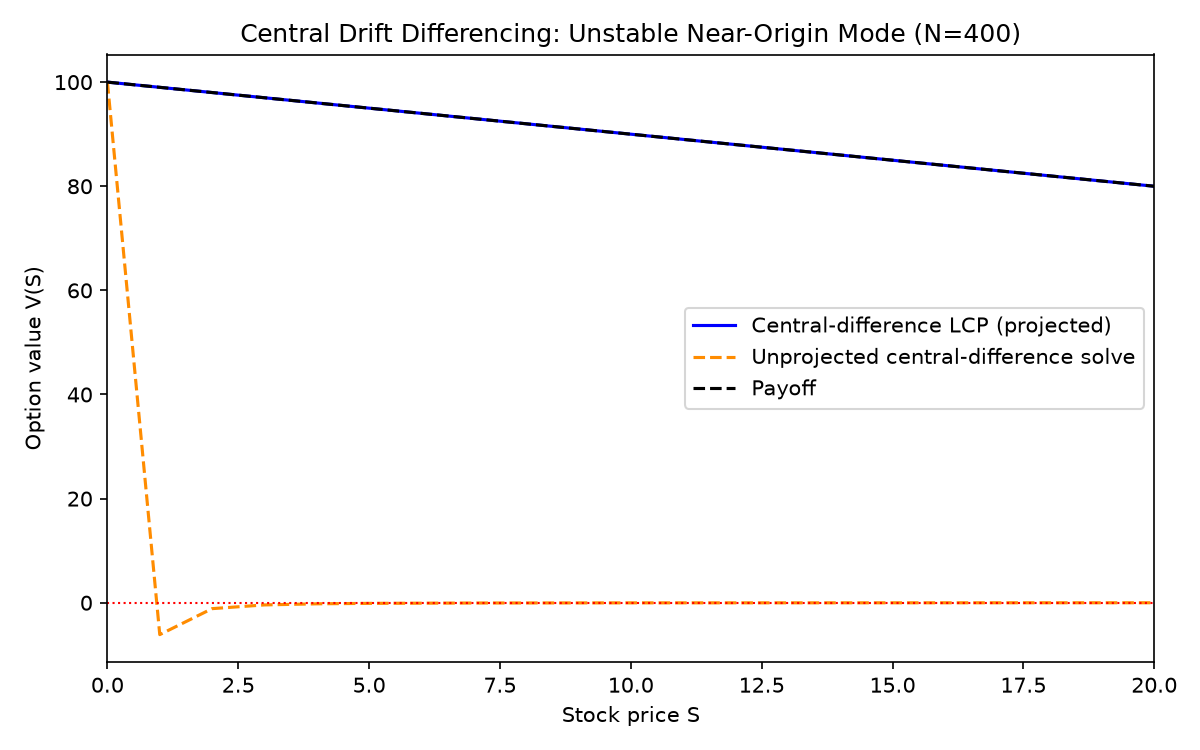
\includegraphics[width=0.92\textwidth]{central_diff_oscillations.png}
\caption{Negative control for central drift differencing at $N=400$ and
$S_{\max}=400$. The unprojected solution develops a negative spike near
$S\approx1$ and a non-monotone boundary layer because the near-origin cell
P\'eclet number exceeds two. The fitted scheme keeps both off-diagonals
non-positive and removes the mode.}
\label{fig:centraldiff}
\end{figure}

\subsection{Discrete Structure}
\label{sec:discrete_structure}
The interior discrete problem is
\begin{equation}
    \min\left((A_hV)_i-F_i,\;V_i-\psi_i\right)=0,
    \qquad i=1,\ldots,N-1,
    \label{eq:discretelcp}
\end{equation}
with the boundary contributions already moved into $F_i$. Equivalently, each
interior node satisfies
\begin{equation}
    a_{h,i}:=(A_hV)_i-F_i\ge0,
    \qquad
    b_{h,i}:=V_i-\psi_i\ge0,
    \qquad
    a_{h,i}b_{h,i}=0.
    \label{eq:discretecomplementarity}
\end{equation}
The first inequality is the differential residual, and the second is the
obstacle slack.

Because $A_h$ is a nonsingular M-matrix, the discrete LCP has a unique
solution. The argument is the standard comparison argument for obstacle
problems. Suppose two admissible vectors satisfy the complementarity
conditions. On rows where one vector is in the continuation region, its
operator residual vanishes; on rows where it touches the obstacle, its value
is fixed by the payoff. Subtracting the two relations and applying the
M-matrix inequality shows that neither vector can exceed the other. The
active set is consequently unique as well.

The two complementary conditions are checked directly from the computed
vectors. In the exercise region one expects $b_h=0$ and $a_h\ge0$; in the
continuation region one expects $b_h>0$ and $a_h=0$. Figure~\ref{fig:lcp_verification}
shows this pattern at $N=400$. The left panel has zero slack up to the
computed boundary and positive slack thereafter. The right panel has a
positive constant residual in the exercise region and a residual at the
level of round-off in the continuation region. The numerical checks also
confirm the off-diagonal signs, diagonal positivity, payoff bounds,
monotonicity, convexity, and contiguity of the contact set.

\begin{figure}[H]
\centering
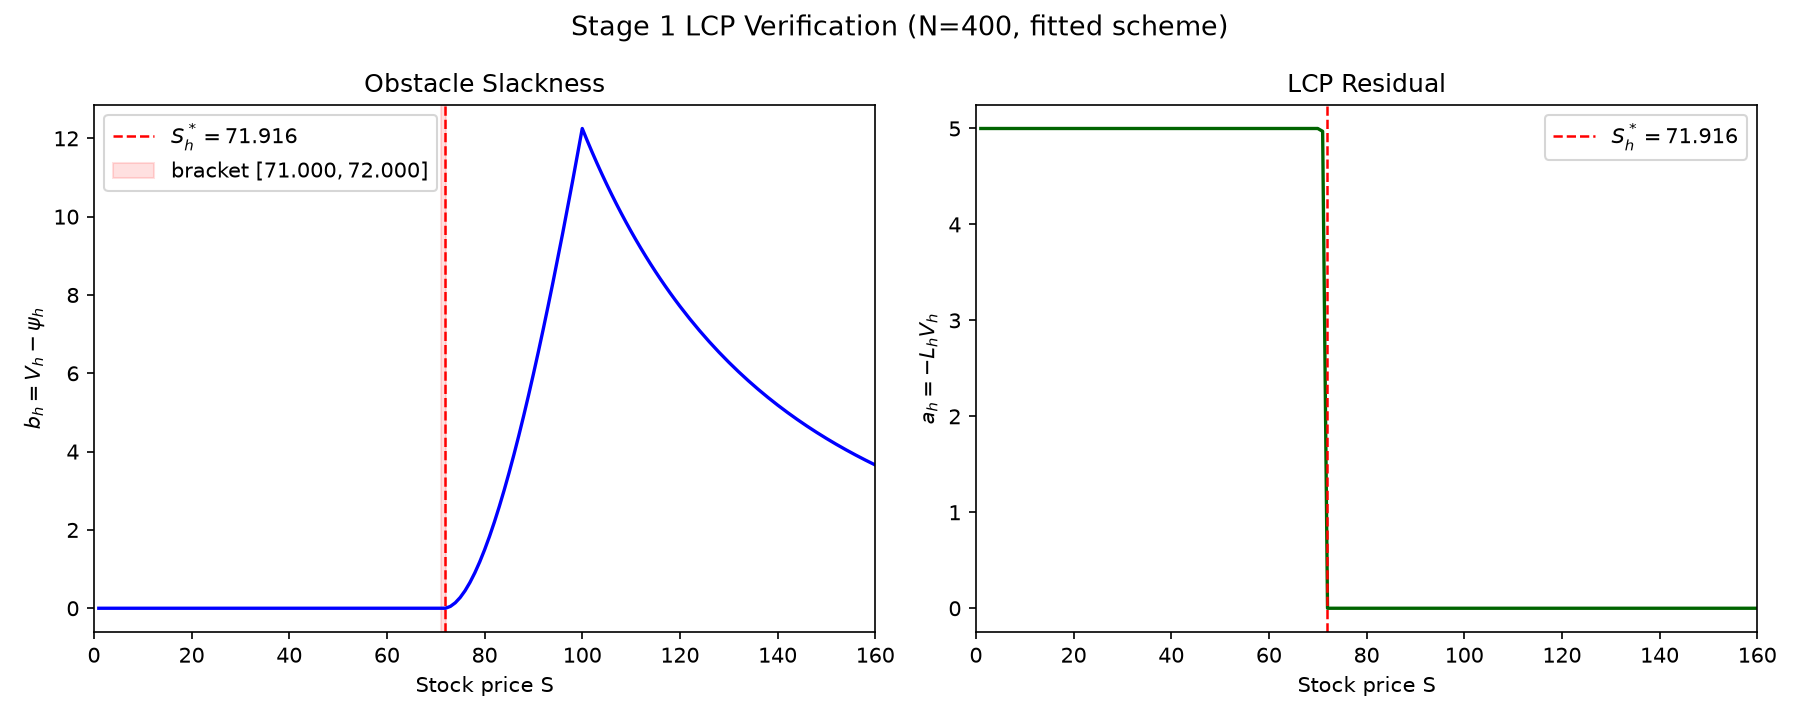
\includegraphics[width=0.98\textwidth]{lcp_verification.png}
\caption{Discrete complementarity at $N=400$ and $S_{\max}=400$. The left
panel shows the obstacle slack $V_h-\psi_h$; the right panel shows the LCP
residual $a_h=A_hV_h-F_h$. Zero slack with a non-negative residual on the
exercise side, and zero residual with positive slack on the continuation
side, verify both complementary conditions.}
\label{fig:lcp_verification}
\end{figure}

The LCP diagnostics used in the remainder of the report are
\begin{equation}
    \min_i a_{h,i},
    \qquad
    \min_i b_{h,i},
    \qquad
    \left\|\min(a_h,b_h)\right\|_\infty,
    \label{eq:diagnostics}
\end{equation}
together with the Boolean checks $\psi_h\le V_h\le K$, monotone decrease, and
convexity. The recent LCP literature uses related residual and active-set
criteria when assessing convergence of splitting and penalty methods
\cite{ref9}. Here the checks are applied on every reported mesh, not only on
the verification mesh.

\begin{figure}[H]
\centering
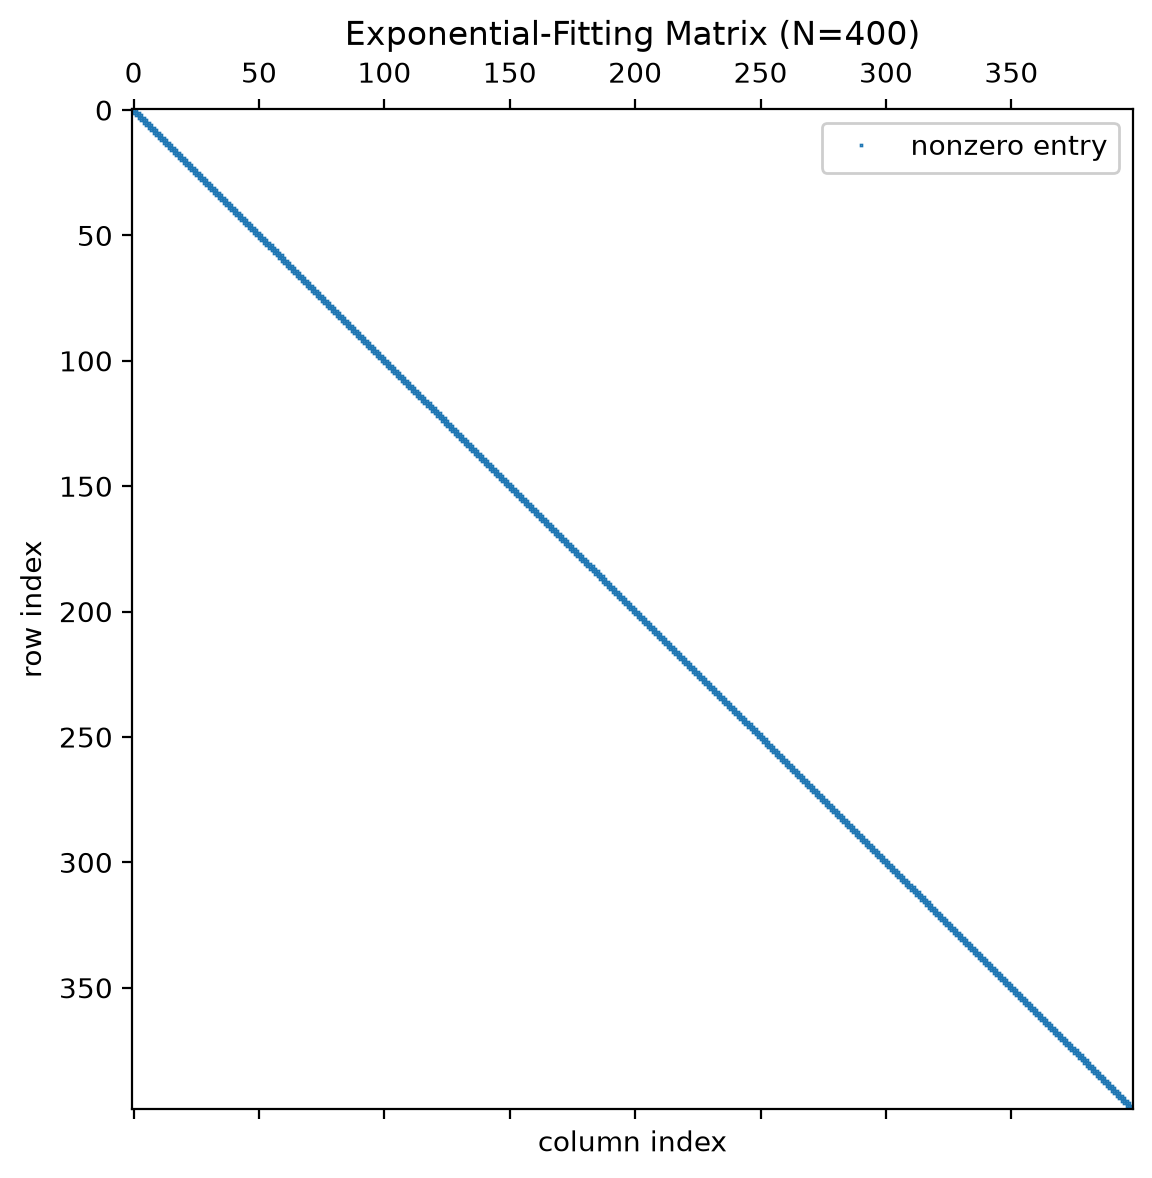
\includegraphics[width=0.5\textwidth]{matrix_spy_fitted_n400.png}
\caption{Sparsity pattern of the assembled system matrix for $N=400$. The
matrix is strictly tridiagonal, allowing sparse direct solvers to operate
efficiently.}
\label{fig:matrix_sparsity}
\end{figure}

As visualized in Figure~\ref{fig:matrix_sparsity}, the assembled system is a
highly sparse tridiagonal matrix. This sparsity is the fundamental reason why
our Policy Iteration approach, which relies on direct sparse solves at each
step, remains extremely efficient.

\subsection{Adaptive Grids, Robin Closure, and Sensitivities}
\label{sec:advanced-methods}
The uniform scheme is the production baseline because it makes the
M-matrix argument transparent. Four extensions remove its main accuracy
bottlenecks without changing the complementarity solver. They are used in
Sections~\ref{sec:adaptive-experiments} and~\ref{sec:sensitivity}.

On a nonuniform grid let
\begin{equation}
    h_i^- = S_i-S_{i-1},
    \qquad
    h_i^+ = S_{i+1}-S_i,
    \qquad
    \bar h_i = \frac{h_i^-+h_i^+}{2},
    \label{eq:nonuniform-spacings}
\end{equation}
and define the directional cell P\'eclet numbers
$\operatorname{Pe}_i^-=b_ih_i^-/a_i$ and
$\operatorname{Pe}_i^+=b_ih_i^+/a_i$. The fitted flux balance gives
\begin{align}
    \ell_i &= -\frac{a_i}{h_i^-\bar h_i}B(\operatorname{Pe}_i^-),
    \label{eq:nonuniform-lower}\\
    u_i &= -\frac{a_i}{h_i^+\bar h_i}B(-\operatorname{Pe}_i^+),
    \label{eq:nonuniform-upper}\\
    d_i &= -\ell_i-u_i+r.
    \label{eq:nonuniform-diagonal}
\end{align}
Because $B(z)>0$, both off-diagonals remain non-positive and
$d_i+\ell_i+u_i=r$, so the M-matrix property is preserved cell by cell. This
is what permits local refinement near the free boundary without a change of
solver or a loss of monotonicity.

In the continuation region at large $S$, the leading solution behaves as
$V\sim C S^\lambda$, where
\begin{equation}
    \lambda=\frac{-\bigl((r-q)-\tfrac12\sigma^2\bigr)
    -\sqrt{\bigl((r-q)-\tfrac12\sigma^2\bigr)^2+2\sigma^2r}}{\sigma^2}.
    \label{eq:robin-lambda}
\end{equation}
Consequently $SV'(S)=\lambda V(S)$ holds asymptotically. Discretising this
relation with the last mesh interval gives
\begin{equation}
    S_{\max}\frac{V_N-V_{N-1}}{h_N^-}
    =\lambda V_N
    \quad\Longrightarrow\quad
    V_N=\frac{S_{\max}}{S_{\max}-\lambda h_N^-}V_{N-1}.
    \label{eq:robin-elimination}
\end{equation}
Eliminating $V_N$ adds $u_{N-1}$ times this ratio to the last diagonal
entry. Since $\lambda<0$ and the ratio is less than one, the modified row
retains a positive diagonal and a non-positive off-diagonal. This closure is
used only at the artificial far boundary; the obstacle problem near $S^*$ is
unchanged.

For the free boundary, the slack satisfies
$b_h(S)=c(S-S^*)^2+O((S-S^*)^3)$ in the continuation region. Writing
$g_h=\sqrt{b_h}$ therefore removes the quadratic behaviour. Instead of the
two-point formula \eqref{eq:interpolation}, we fit a straight line to $g_h$
at the first four continuation nodes by least squares and take its root
inside the bracket. The resulting estimate uses several cells and is less
sensitive to the phase of the free boundary relative to the mesh.

Finally, let $F$ and $A$ denote the free and active interior rows for a
converged policy, and let $I=F\cup A$. Locally differentiating the free-row
equations with respect to a parameter $\theta\in\{r,q,\sigma\}$ gives
\begin{equation}
    A_{FF}\frac{\partial V_F}{\partial\theta}
    =\frac{\partial F_F}{\partial\theta}
    -\frac{\partial A_{FI}}{\partial\theta}V_I,
    \label{eq:adjoint-system}
\end{equation}
because the values on the active set are fixed by the payoff. For a linear
functional $J=w^\top V$, solve the discrete adjoint system
$A_{FF}^\top\lambda_F=w_F$. Then
\begin{equation}
    \frac{\partial J}{\partial\theta}
    =\lambda_F^\top\left(
    \frac{\partial F_F}{\partial\theta}
    -\frac{\partial A_{FI}}{\partial\theta}V_I
    \right).
    \label{eq:adjoint-derivative}
\end{equation}
The same adjoint vector therefore provides the sensitivities to all
parameters; only the right-hand side changes. In the implementation,
$\partial A/\partial\theta$ and $\partial F/\partial\theta$ are evaluated by
centred differences of the assembled operator, while the active/free
partition is held fixed at the converged solution.

\newpage
% ============================================================
\section{Implementation}
\label{sec:implementation}
% ============================================================

\subsection{Algorithm}
\label{sec:algorithm}
Let $\mathcal{A}\subset\{1,\ldots,N-1\}$ denote the current active set, that
is, the nodes at which the obstacle is imposed. A policy step replaces the
equation at active nodes by $V_i=\psi_i$ and removes the couplings from those
nodes to their neighbours. The resulting system is solved for the remaining
values. The residual of the full operator is then evaluated. An active node
whose full residual is negative is released; a continuation node whose value
falls below the obstacle is added. The process is repeated until the policy
is unchanged and the maximum update is below $10^{-12}$.

This is the policy-iteration form of the active-set method introduced by
Howard for Markov decision processes \cite{ref7}. Each iteration solves a
linear system rather than performing a relaxation sweep. Because the policy
space is finite and the matrix is monotone, a repeated policy certifies the
discrete solution. The practical iteration count is small for the present
problem, although the worst-case bound over all active sets is exponential
in the number of nodes and is not a useful complexity estimate.

\begin{algorithm}[H]
\caption{Exponential-fitting LCP solved by policy iteration}
\label{alg:policy}
\begin{algorithmic}[1]
\Require $N$, $K$, $r$, $q$, $\sigma(S)$, $S_{\max}$, payoff $\psi$, tolerance
\Ensure Discrete value $V_h$ and free-boundary estimate $S_h^*$
\State Build the grid $S_i=ih$ and coefficients $a_i,b_i$
\State Compute $\operatorname{Pe}_i=b_ih/a_i$ and the fitted weights
       $\ell_i,d_i,u_i$
\State Assemble $A_h$; move the Dirichlet data to the right-hand side
\State Initialise $V\leftarrow\psi$ and mark every interior row active
\Repeat
    \State Compute the full residual $a_h=A_hV-F_h$
    \State Release active rows whose residual is negative
    \State Set $V_i=\psi_i$ and decouple the neighbouring rows on active rows
    \State Solve the resulting sparse tridiagonal system
    \State Project $V\leftarrow\max(V,\psi)$
    \State Record $\|V^{\mathrm{new}}-V^{\mathrm{old}}\|_\infty$
\Until{the active set is unchanged and the update is below the tolerance}
\State Locate the exercise/continuation bracket and apply
       \eqref{eq:interpolation}
\State \Return $V_h$ and $S_h^*$
\end{algorithmic}
\end{algorithm}

The initial vector is the payoff itself. This choice satisfies the obstacle
constraint and gives a natural starting policy in which every node is active.
The solver then releases the continuation nodes as the residual detects that
continuation is more valuable. No continuation value or analytic free
boundary is used in the iteration.

\subsection{Data Structures and Numerical Details}
\label{sec:implementation-details}

\paragraph{Separation of responsibilities.}
The implementation is split into four layers: a shared fitted-operator and
LCP module, a Stage~2 wrapper, experiment drivers, and plotting utilities.
The core numerical modules return structured objects rather than printing
numbers, so the same solution can feed diagnostics, figures, and the text.
This separation also makes the production path auditable from a single entry
point.

\paragraph{Operator object.}
The dataclass \texttt{GridOperator} in \texttt{stage1\_validation.py} stores
the grid size \texttt{N}, the node array \texttt{S}, the payoff
\texttt{psi}, the three tridiagonal arrays \texttt{lower}, \texttt{diag},
and \texttt{upper}, the right-hand side \texttt{rhs}, the boundary data
\texttt{V\_left} and \texttt{V\_right}, and the mesh width \texttt{h}. The
constructor \texttt{build\_fitted\_operator} uses $h=S_{\max}/N$ and
$N-1$ interior unknowns. The volatility argument accepts a scalar, an
array of length $N-1$, or a callable, so Stage~1 and Stage~2 share exactly
the same assembly and policy-iteration code.

Assembly is vectorised. For each interior node the routine evaluates
$a_i=\tfrac12\sigma_i^2S_i^2$, $b_i=(r-q)S_i$,
$\mathrm{Pe}_i=b_ih/a_i$, and the fitted weights
\eqref{eq:lower}--\eqref{eq:upper}. The Bernoulli factor uses the
three-term Taylor expansion for $|z|<10^{-8}$ and the stable identity
$z/(e^z-1)$ otherwise. The boundary contribution is then moved to
\texttt{rhs}, so no boundary unknown is retained in the linear system. The
matrix is never formed densely: \texttt{\_system\_matrix} calls
\texttt{scipy.sparse.diags(..., format="csr")}, and each policy solve calls
\texttt{scipy.sparse.linalg.spsolve}. Before every solve,
\texttt{\_assert\_m\_matrix} checks that the diagonal is positive and that
the largest off-diagonal is non-positive up to a round-off scale; a
violation raises an exception rather than silently returning a
non-monotone solution.

\paragraph{Result object and solve pipeline.}
The dataclass \texttt{LCPResult} returns the full value vector \texttt{V},
the free-boundary bracket and estimate, the value errors, the policy
iteration count, the final update, and the diagnostics
\texttt{min\_a}, \texttt{min\_b}, \texttt{complementarity},
\texttt{value\_bounds\_ok}, \texttt{monotone}, \texttt{convex}, and
\texttt{single\_contact\_set}. The public routine
\texttt{solve\_perpetual\_american\_put} composes three operations:
operator construction, LCP solution, and post-processing. Stage~2 replaces
the constant $\sigma$ by the callable \eqref{eq:localvol} inside the same
pipeline.

Inside \texttt{solve\_lcp}, a Boolean active mask marks the rows currently
constrained by the obstacle. The solver starts from $V_h=\psi_h$. In each
policy step it evaluates the full residual $a_h=A_hV_h-F_h$, releases an
active row when $a_{h,i}< -10^{-10}$, overwrites the diagonal of every active
row by one, zeros its two adjacent off-diagonals, and replaces its
right-hand side by $\psi_i$. The resulting CSR system is solved directly and
projected back onto the obstacle. The loop ends when
$\max_i|V_i^{\text{new}}-V_i^{\text{old}}|<10^{-12}$ and the active set is
unchanged for two consecutive iterations; the hard limit is $10{,}000$
policy steps. The field \texttt{residual} stores this final update, while the
separate LCP diagnostics provide the algebraic certificate. The fixed
constant \texttt{POLICY\_TOL}=$10^{-10}$ controls active-set membership;
the boundary-classification tolerance is
\texttt{SLACK\_TOL}=$10^{-10}K$.

\paragraph{Post-processing and free-boundary recovery.}
The routine \texttt{lcp\_residuals} evaluates
$a_h=A_hV_h-F_h$ and $b_h=V_h-\psi_h$ on all interior nodes.
\texttt{compute\_lcp\_diagnostics} uses them to compute
$\min_i a_{h,i}$, $\min_i b_{h,i}$,
$\|\min(a_h,b_h)\|_\infty$, the obstacle bounds, monotonicity,
convexity, and single-interval contact-set checks. The free boundary is not
read off as a single grid index. \texttt{extract\_free\_boundary} identifies
the last contact node and the first continuation node, then extrapolates
$\sqrt{b_h}$ through the first two continuation nodes; the square-root
transform is natural because $b_h$ behaves like $c(S-S^*)^2$ locally. The
estimate is clamped to the bracket $[S_{\mathrm{lo}},S_{\mathrm{hi}}]$, with
the bracket midpoint as a fallback. The Stage~2 validation reference is not
built from this routine: \texttt{reference\_solution.py} integrates the
free-boundary ODE directly and is independent of the finite-difference grid.

\paragraph{Two LCP solvers and residual control.}
Policy iteration is the production solver, but it is not the only one.
\texttt{experiment\_solvers.py} implements PSOR on the identical fitted
operator, with the same initial iterate $V_h=\psi_h$, the same relaxation
parameter $\omega=1.2$, and the same tolerance $10^{-10}$. PSOR evaluates
the componentwise complementarity residual every 100 sweeps and stops only
when $\|\min(a_h,b_h)\|_\infty<10^{-10}$; the iterate difference is still
recorded for diagnosis but is not the stopping test. The driver reports the
final update, the true LCP residual, the iteration count, and the CPU time
for both methods. This is the second method used in the report: a genuine
second LCP solver, not merely a second plotting convention. Central
differencing is a separate negative control for the discretisation, not a
competing production solver.

\paragraph{Advanced extensions.}
The module \texttt{advanced\_methods.py} introduces the dataclass
\texttt{NonuniformOperator} and the constructor
\texttt{build\_nonuniform\_operator}. It stores left and right mesh spacings
and builds the nonuniform fitted weights
\eqref{eq:nonuniform-lower}--\eqref{eq:nonuniform-diagonal}. For the Robin
closure, the last diagonal entry is augmented by
$u_{N-1}S_{\max}/(S_{\max}-\lambda h_{\rm last})$, which eliminates the
outgoing tail without enlarging the domain. The same module provides a
four-point square-root extrapolation for $S_h^*$ and a sparse discrete
adjoint solve: after forming $\partial A/\partial\theta$ and
$\partial F/\partial\theta$ by centred differences, one transposed solve
produces the sensitivities to all parameters. None of these extensions
changes the core LCP solver.

\paragraph{Library calls and project code.}
NumPy supplies arrays and vectorised arithmetic; SciPy supplies sparse
assembly (\texttt{diags}) and the direct factorisation (\texttt{spsolve})
\cite{ref5}; Matplotlib supplies the figures. The exponential-fitting weights, the
active-set policy, the M-matrix assertion, the LCP diagnostics, the
free-boundary rule, the nonuniform operator, the Robin elimination, and the
adjoint derivative formula are project code. This division is deliberate:
the libraries provide robust storage and linear algebra, while the
problem-specific discretisation and complementarity logic remain explicit
and modifiable.

Table~\ref{tab:code_structure} lists the production modules and experiment
drivers. The single reproducibility entry point is
\texttt{python run\_all.py}; it executes the scripts in dependency order and
fails if an expected figure or data file is missing.

\begin{table}[H]
\centering
\scriptsize
\setlength{\tabcolsep}{3pt}
\begin{tabular}{@{}>{\raggedright\arraybackslash}p{0.30\textwidth}>{\raggedright\arraybackslash}p{0.64\textwidth}@{}}
\toprule
\textbf{File} & \textbf{Responsibility} \\
\midrule
\texttt{stage1\_validation.py} & Shared fitted operator, policy iteration,
LCP residuals, shape diagnostics, free-boundary extraction, and the Stage~1
closed-form validation. \\
\texttt{stage2\_local\_volatility.py} & Reuses the fitted operator with the
callable local volatility and $q=0.02$; produces the Stage~2 value,
diagnostics, and comparison figure. \\
\texttt{reference\_solution.py} & Independent DOP853 shooting reference for
the infinite-domain and finite-domain free-boundary problems, with a
closed-form self-check for constant volatility. \\
\texttt{grids.py} & Boundary-aligned uniform and clustered validation grids
used to separate the spatial order from the free-boundary phase. \\
\texttt{advanced\_methods.py} & Nonuniform fitted operator, adaptive
clustering, asymptotic Robin closure, four-point boundary extraction, and
discrete adjoint sensitivities. \\
\texttt{experiment\_convergence.py} & Aligned-grid Stage~1 refinement study
plus production-boundary diagnostics; writes
\texttt{stage1\_convergence.csv}. \\
\texttt{experiment\_central\_diff.py} & Negative control for central drift
differencing, including the positive-off-diagonal and oscillation evidence. \\
\texttt{experiment\_solvers.py} & Residual-controlled PSOR benchmark against
policy iteration on the identical fitted LCP; also writes the four-tolerance
sweep to \texttt{tolerance\_sweep.csv}. \\
\texttt{experiment\_smax.py}, \texttt{experiment\_neumann\_true.py}, &
Domain-truncation study, a synthetic zero-flux row stress test, and
independent LCP verification checks; \texttt{experiment\_verification.py}
supplies the reusable residual/shape audit. \\
\texttt{stage2\_convergence\_report.py} & Four-mesh local-volatility study
against the independent ODE reference; writes
\texttt{stage2\_convergence.csv}. \\
\texttt{plot\_matrix\_spy.py} & Builds the $100\times100$ fitted and central
matrices for the spy comparison and the $N=400$ sparsity figure. \\
\texttt{plot\_lcp\_verification.py}, \texttt{plot\_greeks.py}, & Residual,
obstacle-slackness, Delta, and Gamma figures from the computed arrays. \\
\texttt{plot\_solver\_comparison.py}, \texttt{plot\_smax\_study.py} & Solver
timing and fixed-$h$ truncation figures. \\
\texttt{run\_all.py} & Runs every experiment and plotting script and verifies
that all required artifacts exist. \\
\bottomrule
\end{tabular}
\vspace{0.2cm}
\caption{Implementation files. Core solvers, experiment drivers, and
plotting scripts are separated so that each result can be regenerated and
audited independently.}
\label{tab:code_structure}
\end{table}

\subsection{Computational Cost}
For a tridiagonal system of dimension $N-1$, assembly and factorisation are
linear in $N$, and the storage is linear in $N$. A policy iteration therefore
costs $O(N)$ per iteration plus the cost of detecting the active set. By
contrast, PSOR performs $N-1$ scalar updates per sweep and requires many
sweeps to propagate the free-boundary information across the domain. The
comparison in Section~\ref{sec:error-separation} uses the same discrete
operator, the same tolerance, and the same initial vector for both methods.

\newpage
% ============================================================
\section{Verification and Numerical Experiments}
\label{sec:experiments}
% ============================================================

\subsection{Convergence}
\label{sec:convergence}
The constant-volatility convergence study uses $q=0$, $\sigma=0.20$,
$K=100$, $r=0.05$, and $S_{\max}=2400$. The exact free boundary is
$S^*=71.4286$. The grids are $N=600,1200,2400,4800$, with nominal
$h=4,2,1,0.5$. To measure the order of the spatial stencil rather than the
phase of the free-boundary kink, the validation grid deliberately places a
node exactly at $S^*$ and is uniform on each side of it. This is a controlled
stencil verification, not a blind free-boundary recovery test. The asymptotic
Robin closure is used, so the reported aligned error contains discretisation
error but not the $O(1)$ tail value at the artificial boundary.

The production uniform grid still uses $V(S_{\max})=0$. Its full-grid error
is not used to estimate the order because it mixes three different effects:
the exact value at $S_{\max}$ is $V(2400)=4.366\times10^{-3}$ while the
boundary condition imposes zero; the node nearest to $S^*$ changes phase
under refinement; and the first-order boundary-location error is sampled at
different distances from the kink. Those effects explain the earlier
plateau in the uniform-grid maximum norm and are removed from the aligned
validation sequence. The production contact brackets themselves are retained
in Table~\ref{tab:stage1-production}; they show why a coarse active set cannot
serve as a pointwise boundary estimator. The aligned error is
\begin{equation}
    E_N=\max_{0\le i\le N}|V_i-V(S_i)|,
    \label{eq:maxerror}
\end{equation}
where $V(S_i)$ is the closed-form solution \eqref{eq:exactvalue}.

\begin{table}[H]
\centering
\scriptsize
\setlength{\tabcolsep}{5pt}
\begin{tabular}{ccccccc}
\toprule
\textbf{Grid $N$} & \textbf{$h$} & \textbf{Aligned error $E_N$} &
\textbf{Error ratio} & \textbf{Observed $p$} &
\textbf{LCP res.} & \textbf{tol.} \\
\midrule
$600$  & $4.0$ & $1.0732\times10^{-2}$ & ---     & ---     &
$2.84\times10^{-14}$ & $10^{-10}$ \\
$1200$ & $2.0$ & $2.6895\times10^{-3}$ & $3.990$ & $1.997$ &
$2.27\times10^{-13}$ & $10^{-10}$ \\
$2400$ & $1.0$ & $6.7222\times10^{-4}$ & $4.001$ & $2.000$ &
$9.10\times10^{-13}$ & $10^{-10}$ \\
$4800$ & $0.5$ & $1.6818\times10^{-4}$ & $3.997$ & $1.999$ &
$5.46\times10^{-12}$ & $10^{-10}$ \\
\bottomrule
\end{tabular}
\caption{Stage~1 convergence for constant volatility with $q=0$ on a
free-boundary-aligned validation grid. A node is placed at the exact
$S^*=71.428571$, and the asymptotic Robin closure is used. The error ratios
are $3.990$, $4.001$, and $3.997$, giving observed orders $1.997$, $2.000$,
and $1.999$. The LCP residual is $\|\min(a_h,b_h)\|_\infty$; the policy
update additionally satisfies $\max|dV|<10^{-12}$.}
\label{tab:stage1}
\end{table}

\begin{table}[H]
\centering
\scriptsize
\setlength{\tabcolsep}{5pt}
\begin{tabular}{cccccc}
\toprule
\textbf{$N$} & \textbf{$h$} & \textbf{Production contact bracket} &
\textbf{$S_h^*$} & \textbf{$|S_h^*-S^*|$} & \textbf{Production $E_N$} \\
\midrule
$600$  & $4.0$ & $[72.0,76.0]$ & $72.000$ & $5.714\times10^{-1}$ &
$7.905\times10^{-3}$ \\
$1200$ & $2.0$ & $[72.0,74.0]$ & $72.000$ & $5.714\times10^{-1}$ &
$7.905\times10^{-3}$ \\
$2400$ & $1.0$ & $[71.0,72.0]$ & $71.654$ & $2.254\times10^{-1}$ &
$4.366\times10^{-3}$ \\
$4800$ & $0.5$ & $[71.5,72.0]$ & $71.500$ & $7.143\times10^{-2}$ &
$4.366\times10^{-3}$ \\
\bottomrule
\end{tabular}
\caption{Production uniform-grid diagnostics with $V(S_{\max})=0$. The
``contact bracket'' is the discrete transition from the last active node to
the first continuation node, not a confidence interval. At $N=600$,
$N=1200$, and $N=4800$ the contact set has moved to the right of $S^*$, so
the bracket does not contain the analytic boundary. Only the $N=2400$
bracket does.
Production $E_N$ is the full-grid infinity norm against the closed form;
neither this column nor the individual $S_h^*$ values is used to estimate the
spatial order.}
\label{tab:stage1-production}
\end{table}

The largest LCP residual is $5.46\times10^{-12}$ at $N=4800$, more than
seven orders of magnitude below the corresponding value error. Thus the
reported error is not produced by an incomplete linear solve. Since
\texttt{spsolve} is a direct factorisation, no solver tolerance can be
tightened. Its complementarity residual is therefore reported directly, while
the residual-controlled PSOR solver supplies the tolerance sweep in
Section~\ref{sec:error-separation}.

The ratios in Table~\ref{tab:stage1} are now consistent with a second-order
method: halving $h$ reduces the aligned maximum error by almost exactly a
factor of four. The earlier non-monotone ratios were not a property of the
fitted stencil. They arose because the maximum was attained at the right
boundary, where the exact tail is nonzero, or at a node whose distance to
the free-boundary kink did not halve with the mesh. Separating those effects
recovers the expected order and makes the refinement evidence auditable.

The free-boundary plot in Figure~\ref{fig:freeboundary} uses the production
uniform $N=2400$ solution. Its computed bracket is $[71.00,72.00]$, and the
interpolated estimate lies inside it. At $N=600$ and $N=1200$ the coarse
contact set lies entirely to the right of $S^*$; at $N=4800$ the bracket
$[71.5,72]$ also starts one half-cell to the right. Why the finest mesh still
misses is visible in the slack: the interpolated estimate is clamped to the
lower contact node. This is an active-set localisation error, not a failure
of complementarity: the discrete obstacle and sign constraints remain
satisfied. The exact boundary and each computed bracket are shown separately
so that the aligned validation grid is not mistaken for a blind production
reconstruction.

\begin{figure}[H]
\centering
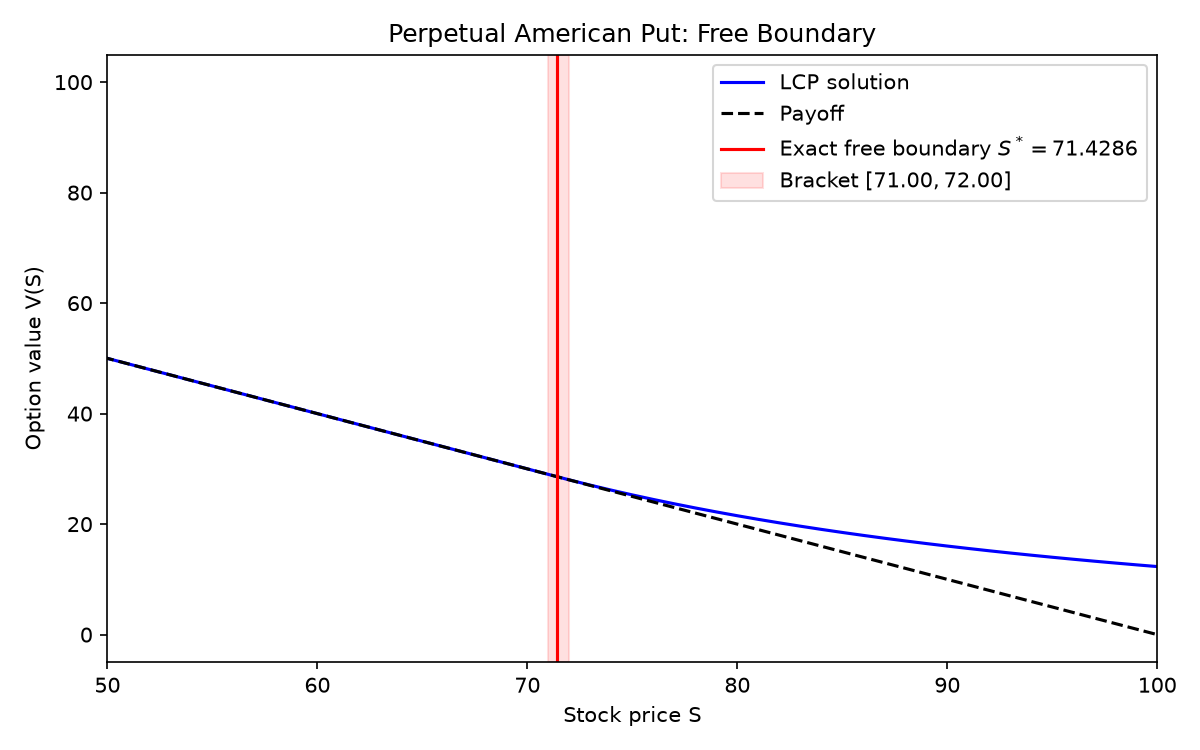
\includegraphics[width=0.92\textwidth]{free_boundary_plot.png}
\caption{Stage~1 value and free boundary at $N=2400$ on $[50,100]$. The
exact boundary $S^*=71.4286$ lies inside the computed bracket
$[71.00,72.00]$. The blue value curve coincides with the payoff on the
exercise side and departs from it in the continuation region. This matters
because it verifies that the obstacle solve recovers the correct exercise and
continuation regions, not merely a smooth-looking value curve.}
\label{fig:freeboundary}
\end{figure}

\subsection{Adaptive Refinement and Far-Field Closure}
\label{sec:adaptive-experiments}
The first experiment compares the uniform grid with a smoothly clustered
grid at the same number of intervals. Both grids contain a node exactly at
the analytic boundary $S^*=71.428571$. The clustering density on the right
of the boundary is $\rho(S)=1+16\exp[-((S-S^*)/15)^2]$, and the grid is
obtained by inverting its cumulative density while retaining the boundary
node. The nonuniform coefficients
\eqref{eq:nonuniform-lower}--\eqref{eq:nonuniform-diagonal} are used on both
grids, and the asymptotic Robin closure \eqref{eq:robin-elimination}
replaces $V(S_{\max})=0$.

Table~\ref{tab:adaptive} shows the expected regular pattern. Halving the
mesh reduces the maximum error on the clustered grid by factors
$3.982$, $4.002$, and $3.999$, giving observed orders $1.993$, $2.001$,
and $2.000$. The uniform/clustered advantage is essentially constant at
$2.25$, because both sequences now resolve the kink at the same phase; the
clustered mesh simply has a smaller local error constant near
$S^*$. The four-point boundary error also falls by approximately a factor
of four on each refinement.

\begin{table}[H]
\centering
\resizebox{\textwidth}{!}{%
\begin{tabular}{ccccccc}
\toprule
\textbf{$N$} & \textbf{Uniform $E_N$} & \textbf{Clustered $E_N$} &
\textbf{Clustered ratio} & \textbf{Observed $p$} &
\textbf{Uniform/clustered gain} & \textbf{Clustered 4-pt error} \\
\midrule
$600$  & $1.0732\times10^{-2}$ & $4.7508\times10^{-3}$ & ---     & ---     &
$2.259$ & $3.067\times10^{-3}$ \\
$1200$ & $2.6895\times10^{-3}$ & $1.1931\times10^{-3}$ & $3.982$ & $1.993$ &
$2.254$ & $7.463\times10^{-4}$ \\
$2400$ & $6.7222\times10^{-4}$ & $2.9809\times10^{-4}$ & $4.002$ & $2.001$ &
$2.255$ & $1.836\times10^{-4}$ \\
$4800$ & $1.6818\times10^{-4}$ & $7.4545\times10^{-5}$ & $3.999$ & $2.000$ &
$2.256$ & $4.553\times10^{-5}$ \\
\bottomrule
\end{tabular}%
}
\caption{Uniform versus clustered grids at equal $N$ with a node at the
analytic free boundary and the asymptotic Robin closure. The clustered
error ratios are $3.982$, $4.002$, and $3.999$, so the observed order is
two. The clustered boundary error uses the four-point $\sqrt{b_h}$
extrapolation.}
\label{tab:adaptive}
\end{table}

The Ratio column now reports the error ratio of the clustered sequence under
mesh halving, rather than a cross-grid ratio whose value has no convergence
meaning. The uniform/clustered gain is shown in a separate column and is
stable at about $2.25$. This separation makes both quantities interpretable:
one measures an order, the other measures the constant-factor benefit of
clustering.

The second experiment isolates far-field truncation. The mesh spacing is
fixed at $h=0.5$ and $S_{\max}$ is varied from $100$ to $800$. The target
price is $S=80$, whose exact value is $V(80)=21.5222117$. The Robin closure
uses the leading decaying tail \eqref{eq:robin-lambda}--\eqref{eq:robin-elimination}.
Table~\ref{tab:robin} shows that the zero-Dirichlet condition can lose more
than one unit of value on a short domain, whereas the Robin condition keeps
the error near $10^{-2}$ at the same mesh spacing. At $S_{\max}=400$ the
reduction is almost three orders of magnitude. The residual Robin error at
$S_{\max}=800$ is dominated by the spatial discretisation, not by the far
tail.

\begin{table}[H]
\centering
\begin{tabular}{ccccc}
\toprule
\textbf{$S_{\max}$} & \textbf{$N$} & \textbf{Dirichlet error} &
\textbf{Robin error} & \textbf{Reduction} \\
\midrule
$100$ & $200$ & $1.522\times10^{0}$ & $2.013\times10^{-2}$ & $75.6$ \\
$150$ & $300$ & $7.446\times10^{-1}$ & $3.267\times10^{-3}$ & $227.9$ \\
$200$ & $400$ & $2.823\times10^{-1}$ & $9.127\times10^{-4}$ & $309.3$ \\
$400$ & $800$ & $2.507\times10^{-2}$ & $6.423\times10^{-5}$ & $390.2$ \\
$800$ & $1600$ & $2.188\times10^{-3}$ & $2.679\times10^{-5}$ & $81.7$ \\
\bottomrule
\end{tabular}
\caption{Far-field closure at fixed $h=0.5$ and target $S=80$. The
asymptotic Robin condition removes most of the domain-truncation error and
requires no extension of the computational domain.}
\label{tab:robin}
\end{table}

\begin{figure}[H]
\centering
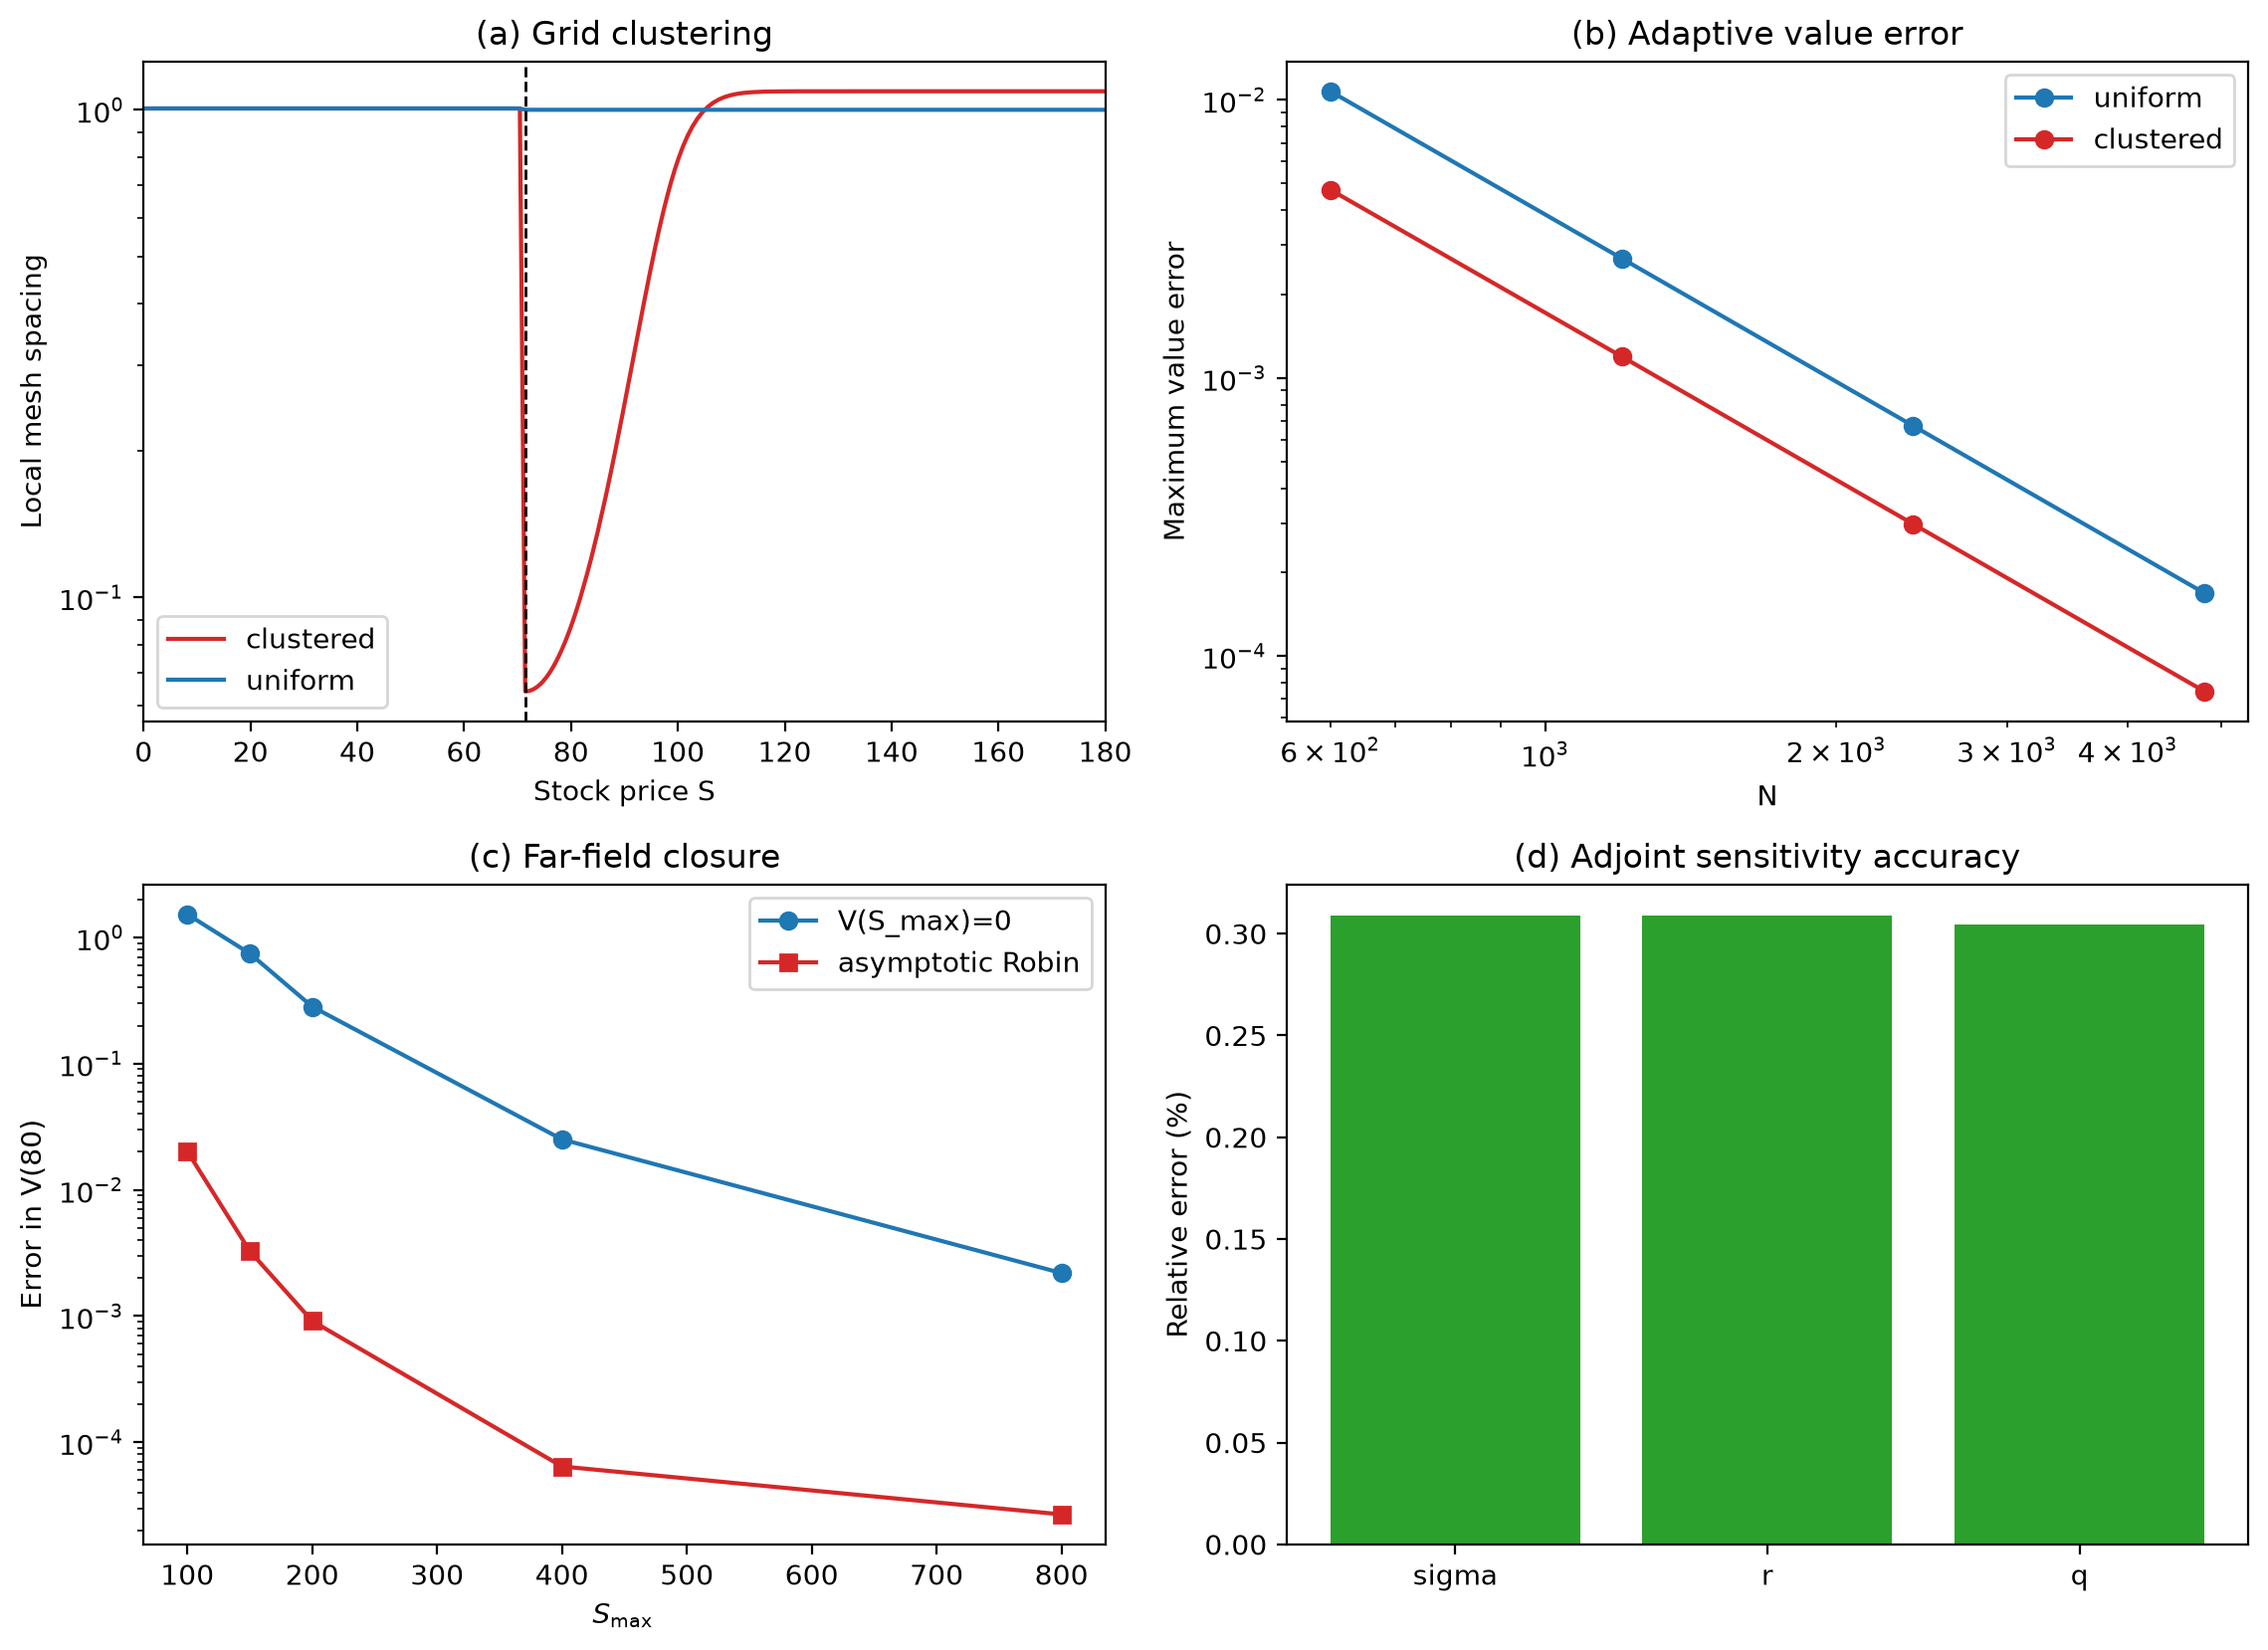
\includegraphics[width=0.98\textwidth]{advanced_methods.png}
\caption{Advanced numerical extensions. (a) The clustered grid concentrates
nodes near the free boundary. (b) Maximum value error versus $N$ for uniform
and clustered grids. (c) Far-field error in $V(80)$ for zero Dirichlet and
asymptotic Robin closures. (d) Relative error of the discrete adjoint
sensitivities at $S=100$ and $N=4800$. The four panels test separate error
sources, so this matters as evidence that each extension improves the quantity
it targets without changing the core LCP solver.}
\label{fig:advanced_methods}
\end{figure}

\subsection{Error Separation}
\label{sec:error-separation}
The algebraic error is separated from the discretisation and truncation
errors by solving the same fitted LCP with two different methods. The
benchmark uses $N=400$, $S_{\max}=400$, $q=0$, $\sigma=0.20$,
$\omega=1.2$, and tolerance $10^{-10}$. PSOR stops on the complementarity
residual and requires 96{,}600 sweeps and $20.635$~s. Policy iteration
requires 301 iterations and $0.045$~s. Its stable-policy certificate gives a
final LCP residual of $9.095\times10^{-13}$; the PSOR residual is
$9.913\times10^{-11}$. The two discrete solutions differ by
$5.685\times10^{-10}$ in the maximum norm. The solution difference is
therefore far below the spatial and truncation errors reported on the
convergence grids.

\begin{table}[H]
\centering
\scriptsize
\resizebox{\textwidth}{!}{%
\begin{tabular}{lccccc}
\toprule
\textbf{Solver} & \textbf{Iterations} & \textbf{CPU time (s)} &
\textbf{Final update} & \textbf{LCP residual} &
\textbf{Max difference} \\
\midrule
Policy iteration & $301$ & $0.045$ & $0$ &
$9.095\times10^{-13}$ & $0$ \\
PSOR ($\omega=1.2$) & $96{,}600$ & $20.635$ & $1.283\times10^{-13}$ &
$9.913\times10^{-11}$ & $5.685\times10^{-10}$ \\
\bottomrule
\end{tabular}
}
\caption{Solver comparison at $N=400$ and matched LCP tolerance. The
iteration ratio is $321$, the wall-time ratio is $4.6\times10^2$, and the
solution difference is negligible relative to the discretisation error.
PSOR uses the residual stopping test; policy iteration reports the LCP
residual obtained from its stable active set.}
\label{tab:solvers}
\end{table}

Two conclusions follow. First, the remaining discrepancy from the
closed-form solution is not caused by an incomplete linear solve. Second,
the free-boundary bracket is stable under a change of algebraic solver. The
comparison supports the error decomposition \eqref{eq:errorbound}: the
dominant errors are spatial and far-field errors, not inner-solver error.
The log-scale presentation in Figure~\ref{fig:solvers} makes the two ratios
visible; the wall-time ratio is hardware-dependent, so the iteration count
is the more portable measure of algorithmic work.

\begin{figure}[H]
\centering
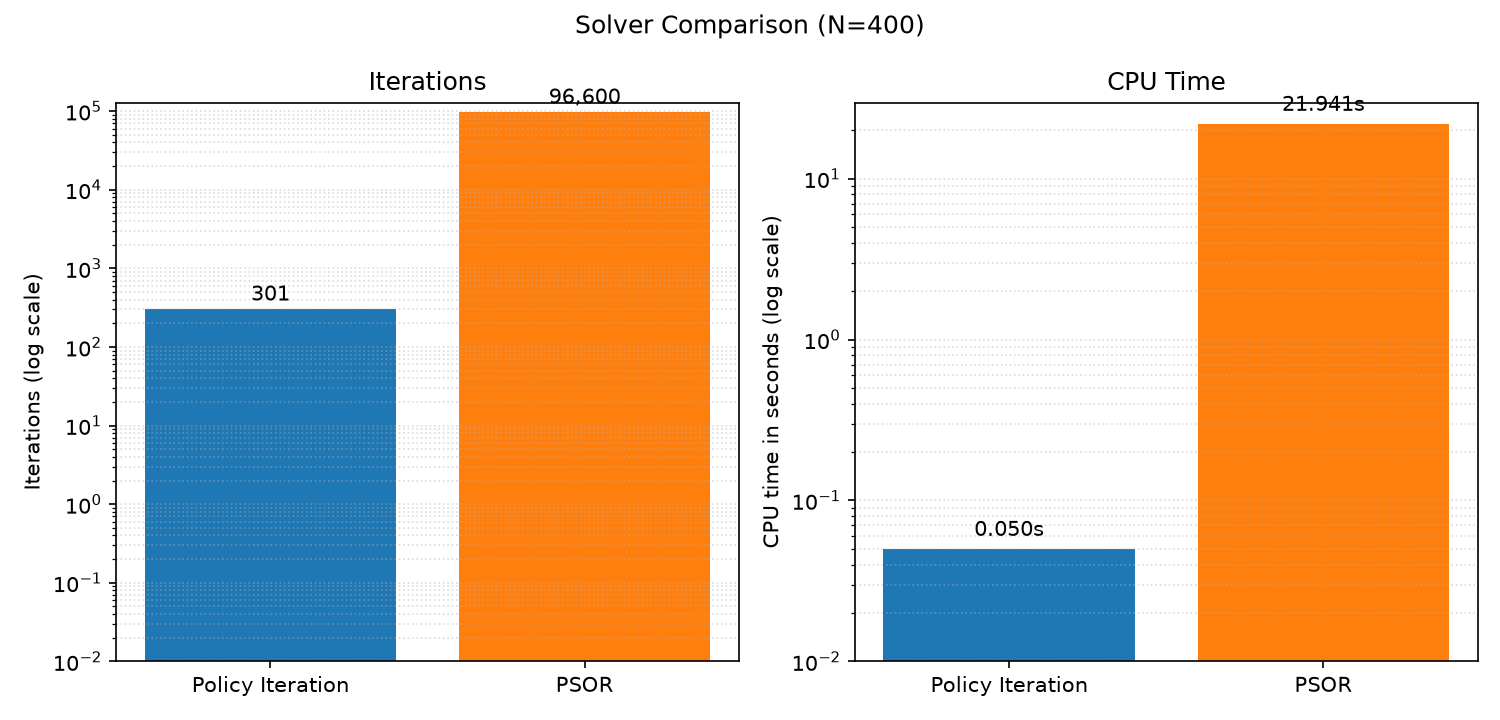
\includegraphics[width=0.96\textwidth]{solver_comparison.png}
\caption{Policy iteration versus PSOR at matched LCP tolerance. Policy
iteration needs 301 iterations and $0.045$~s, while PSOR requires 96{,}600
iterations and $20.635$~s. The logarithmic axes expose the 321-fold
reduction in iterations and the $4.6\times10^2$ reduction in wall time
measured for this experiment.}
\label{fig:solvers}
\end{figure}

\paragraph{Tolerance sweep on one representative mesh.}
The solver comparison establishes that two independent algebraic solvers
agree, but it does not by itself show that the selected stopping tolerance is
below the discretisation error. We therefore fix the same $N=400$,
$S_{\max}=400$ problem and run the residual-controlled PSOR solver at
$\varepsilon=10^{-4},10^{-6},10^{-8},10^{-10}$. The direct policy-iteration
solution is held fixed as the reference because \texttt{spsolve} has no
separate outer tolerance.

Table~\ref{tab:tolerance-sweep} shows the required plateau. At
$\varepsilon=10^{-4}$ both $V(100)$ and $S_h^*$ are visibly shifted. By
$\varepsilon=10^{-8}$, $V(100)$ agrees with the direct reference to
$2.951\times10^{-8}$ and $S_h^*$ is $71.91594$. Tightening once more to
$10^{-10}$ changes $V(100)$ by only $2.953\times10^{-10}$ and changes the
largest nodal value by $5.685\times10^{-10}$. The contact bracket remains
$[71,72]$ at every tolerance. Thus the main quantity and the contact set stop
changing before the tightest setting.

The raw residual is $\|\min(a_h,b_h)\|_\infty$. The scaled residual divides it
by
$\|A_h\|_\infty\|V_h\|_\infty+\|F_h\|_\infty+\|\psi_h\|_\infty$,
so the same measure can be compared across meshes and tolerances. It falls
from $7.858\times10^{-11}$ to $7.901\times10^{-17}$ over the sweep. At the
selected tolerance $10^{-10}$, the algebraic difference is more than five
orders of magnitude below the smallest discretisation error in
Table~\ref{tab:stage1}; changing the stop tolerance below this point cannot
account for any reported convergence or truncation result.

\begin{table}[H]
\centering
\scriptsize
\setlength{\tabcolsep}{4pt}
\resizebox{\textwidth}{!}{%
\begin{tabular}{cccccccc}
\toprule
\textbf{Tolerance} & \textbf{PSOR sweeps} & \textbf{$V(100)$} &
\textbf{$S_h^*$} & \textbf{Raw residual} & \textbf{Scaled residual} &
\textbf{$|\Delta V(100)|$} & \textbf{$\max|\Delta V|$} \\
\midrule
$10^{-4}$ & $35{,}400$ & $12.25111512$ & $71.9183$ &
$9.859\times10^{-5}$ & $7.858\times10^{-11}$ &
$2.947\times10^{-4}$ & $5.675\times10^{-4}$ \\
$10^{-6}$ & $55{,}800$ & $12.25140688$ & $71.9160$ &
$9.865\times10^{-7}$ & $7.863\times10^{-13}$ &
$2.949\times10^{-6}$ & $5.678\times10^{-6}$ \\
$10^{-8}$ & $76{,}200$ & $12.25140980$ & $71.9159$ &
$9.871\times10^{-9}$ & $7.867\times10^{-15}$ &
$2.951\times10^{-8}$ & $5.682\times10^{-8}$ \\
$10^{-10}$ & $96{,}600$ & $12.25140983$ & $71.9159$ &
$9.913\times10^{-11}$ & $7.901\times10^{-17}$ &
$2.953\times10^{-10}$ & $5.685\times10^{-10}$ \\
\bottomrule
\end{tabular}%
}
\caption{PSOR tolerance sweep at $N=400$ and $S_{\max}=400$. The reference is
the direct policy-iteration solution $V_{\mathrm{ref}}(100)=12.2514098322$;
the two difference columns compare against that reference. $V(100)$ and
$S_h^*$ stop changing at the displayed precision, and the bracket remains
$[71,72]$ throughout. This matters because it identifies $10^{-10}$ as a
tolerance safely below the discretisation error, so the reported convergence
and truncation conclusions are not controlled by algebraic stopping error.}
\label{tab:tolerance-sweep}
\end{table}

\subsection{Local Volatility}
\label{sec:localvol}
The local-volatility experiment replaces $\sigma=0.20$ by
\eqref{eq:localvol} and sets $q=0.02$. The dividend yield raises the
opportunity cost of holding the option and therefore lowers the exercise
boundary when volatility is constant. For constant $\sigma=0.20$ and
$q=0.02$, the exact formula \eqref{eq:exactboundary} gives $S^*=64.9219$.
The local-volatility profile is lower than $0.20$ around the boundary, which
reduces the continuation premium and partially offsets the dividend effect.
The mechanism is consistent with the implicit finite-difference
local-volatility framework of \cite{ref8}.
An independent DOP853 shooting solution of the free-boundary ODE gives
\begin{equation}
    S^*=69.1664297389,
    \qquad
    V(100)=16.2054760891,
    \qquad
    V(2400)=4.832780\times10^{-1}
    \label{eq:stage2-reference}
\end{equation}
for the half-line problem. On the finite domain with the production
condition \(V(S_{\max})=0\), the same shooting construction gives
\(S^*=69.1701793435\) and \(V(100)=16.1998980578\). The production solve at
\(N=2400\) gives \(S_h^*=69.1688\) inside the bracket \([69.00,70.00]\).
The coarse \(N=1200\) contact bracket is \([70.00,72.00]\), which does not
contain the finite-domain reference; this case is kept visible in
Table~\ref{tab:stage2-convergence} below.
Relative to the \(q=0\) benchmark \(71.4286\), the boundary is lower;
relative to the constant-volatility, \(q=0.02\) benchmark \(64.9219\), it
is higher. Both comparisons are meaningful, but they answer different
questions.

\subsubsection{Four-Mesh Convergence Against the ODE Reference}
\label{sec:stage2-convergence}
No closed-form solution is available for the chosen local-volatility
profile, but a finer finite-difference solution is no longer used as the
reference. The validation reference is the semi-analytic solution obtained
by shooting the free-boundary ODE with $V(S^*)=K-S^*$ and $V'(S^*)=-1$.
For the infinite-domain value the far field is closed by the decaying
asymptotic Robin condition; for the finite-domain value the production
condition \(V(S_{\max})=0\) is imposed. The ODE integration uses DOP853 with
relative tolerance $10^{-12}$ and absolute tolerance $10^{-14}$. Thus the
reference is independent of the finite-difference stencil and of the
$N=9600$ grid used previously. As a check of the ODE implementation, setting
the local-volatility function to the constant $0.20$ and $q=0$ reproduces the
closed-form boundary to $4.4\times10^{-13}$ and $V(100)$ to
$5.8\times10^{-12}$.

Table~\ref{tab:stage2-convergence} reports two quantities. The production
uniform-grid error is measured against the exact finite-domain reference.
The aligned-validation error places a node at the shooting boundary, so the
free-boundary phase is removed and the observed order can be read directly.

\begin{table}[H]
\centering
\scriptsize
\setlength{\tabcolsep}{3pt}
\begin{tabular}{cccccccc}
\toprule
\textbf{$N$} & \textbf{$h$} & \textbf{Production $E_N$} &
\textbf{Aligned $E_N$} & \textbf{Aligned ratio} & \textbf{Observed $p$} &
\textbf{Production bracket} & \textbf{Production $S_h^*$} \\
\midrule
$600$  & $4.0$  & $2.7701\times10^{-2}$ & $3.2218\times10^{-2}$ & ---     & ---     & $[68.0,72.0]$ & $69.167$ \\
$1200$ & $2.0$  & $2.2835\times10^{-2}$ & $8.0948\times10^{-3}$ & $3.980$ & $1.993$ & $[70.0,72.0]$ & $70.000$ \\
$2400$ & $1.0$  & $1.5248\times10^{-3}$ & $2.0239\times10^{-3}$ & $4.000$ & $2.000$ & $[69.0,70.0]$ & $69.169$ \\
$4800$ & $0.5$  & $9.4068\times10^{-4}$ & $5.0610\times10^{-4}$ & $3.999$ & $2.000$ & $[69.0,69.5]$ & $69.228$ \\
\bottomrule
\end{tabular}
\caption{Local-volatility convergence against the independent ODE shooting
reference. Production errors use the uniform solver; aligned errors use a
grid with a node at the finite-domain shooting boundary. The aligned ratios
are $3.980$, $4.000$, and $3.999$, so the spatial order is two. The finite
reference is \(S^*=69.1701793435\); the infinite-domain reference is
\(S^*=69.1664297389\). The bracket at $N=1200$ does not contain the finite
reference, so the production brackets are reported as discrete contact sets
and are not used to infer an order or a monotone boundary-recovery rate.}
\label{tab:stage2-convergence}
\end{table}

The production error decreases overall, but its successive ratios are
$1.21$, $14.98$, and $1.62$, rather than approaching four. This happens
because the free-boundary kink crosses a different position relative to the
uniform nodes on each mesh and because the contact set is poorly localised at
the coarser resolutions; it is not evidence of first-order consistency in the
smooth region. The aligned sequence removes the phase and gives
$p=1.993,2.000,2.000$, which is the expected second-order rate. The
$N=1200$ contact set is displaced one node to the right
(\(70.000-69.170=0.830<h=2.0\)); the discrete complementarity residual
remains small, so this is a coarse contact-set localisation error rather than
an algebraic failure. The finite and infinite-domain references differ by
$3.750\times10^{-3}$ in the boundary and by $5.578\times10^{-3}$ in
\(V(100)\). At the production mesh $N=2400$ ($h=1$), the error against the
finite-domain reference is $1.5248\times10^{-3}$, while the total error
against the infinite-domain value is $4.055\times10^{-3}$. The latter is not
the pure truncation error: truncation contributes $5.578\times10^{-3}$ and
discretisation partially cancels it. The far-edge gap is
$4.833\times10^{-1}$, so it is quantified separately below.

\begin{figure}[H]
\centering
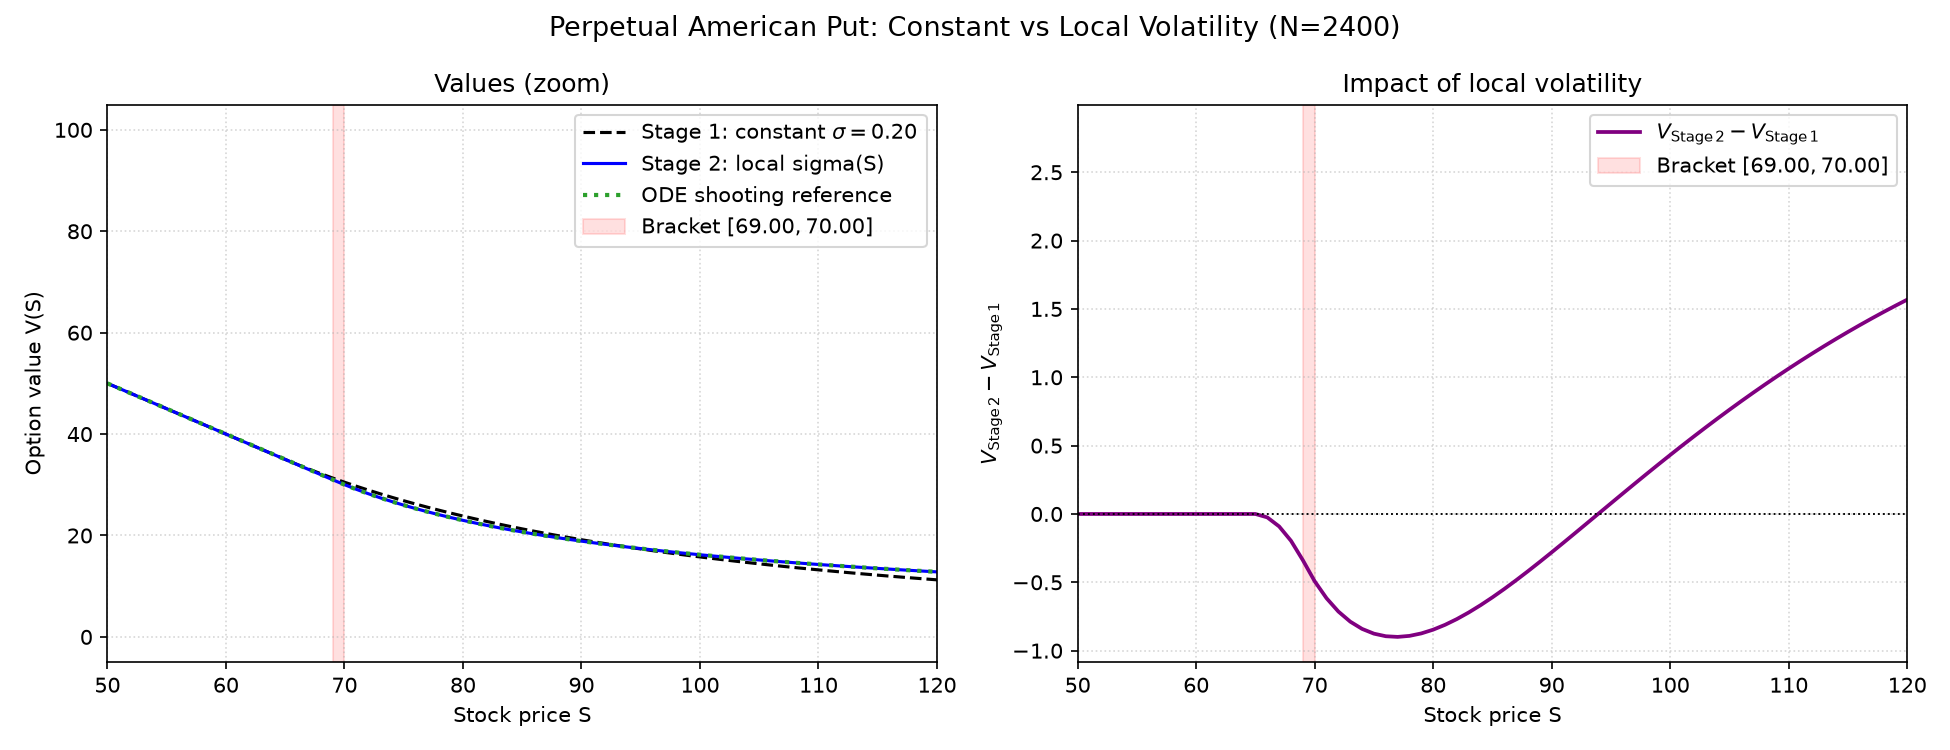
\includegraphics[width=0.96\textwidth]{stage2_plot.png}
\caption{Constant versus local volatility at $N=2400$ with $q=0.02$. The
left panel compares the value functions on $[50,120]$ and includes the
independent ODE shooting reference; the right panel shows
$V_{\mathrm{local}}-V_{\mathrm{const}}$. The difference is zero in the
common exercise region, negative in an interval around $70$--$90$, and
positive at high prices. The shaded band is the computed local-volatility
bracket $[69,70]$. This matters because it shows that the local-volatility
profile changes the price away from the constant-volatility benchmark while
remaining consistent with the independent reference near the boundary.}
\label{fig:stage2}
\end{figure}

\subsubsection{LCP and Shape Diagnostics}
\label{sec:stage2-diagnostics}
Table~\ref{tab:stage2-diagnostics} reports the residual and shape checks on
all four meshes. The smallest slack $b_h=V_h-\psi_h$ is exactly zero, so no
node violates the obstacle. The minimum differential residual remains
slightly negative, at worst $-1.164\times10^{-10}$; this is the policy
iteration tolerance rather than a violation of the continuous
complementarity condition. The norm of the complementarity residual increases
with $N$ but stays below $10^{-9}$ on every mesh. The value bounds,
monotonicity, convexity, and single-interval contact-set checks all pass.

\begin{table}[H]
\centering
\scriptsize
\setlength{\tabcolsep}{4pt}
\begin{tabular}{cccccccc}
\toprule
\textbf{$N$} & \textbf{$\min a_h$} & \textbf{$\min b_h$} &
\textbf{$\|\min(a_h,b_h)\|_\infty$} & \textbf{Bounds} &
\textbf{Monotone} & \textbf{Convex} & \textbf{One contact set} \\
\midrule
$600$  & $-1.364\times10^{-12}$ & $0$ & $1.364\times10^{-12}$ &
True & True & True & True \\
$1200$ & $-3.638\times10^{-12}$ & $0$ & $5.457\times10^{-12}$ &
True & True & True & True \\
$2400$ & $-2.183\times10^{-11}$ & $0$ & $2.183\times10^{-11}$ &
True & True & True & True \\
$4800$ & $-1.164\times10^{-10}$ & $0$ & $1.164\times10^{-10}$ &
True & True & True & True \\
\bottomrule
\end{tabular}
\caption{LCP residual and solution-shape diagnostics for the local-volatility
problem. The contact set is the single interval $[0,S_h^*]$. The worst
complementarity residual is $1.164\times10^{-10}$, below the stated
tolerance $10^{-9}$.}
\label{tab:stage2-diagnostics}
\end{table}

These checks are important because the local-volatility reference is
semi-analytic rather than a closed-form formula. The figure, the residual
checks, and the independent ODE solution therefore supply three distinct
forms of evidence.

The domain-truncation study holds $h=1$ fixed and varies $S_{\max}$ from
$300$ to $2400$. The values of $V(100)$ are reported in
Table~\ref{tab:smax}. Because the mesh spacing is unchanged, the residual
difference isolates the effect of replacing the decaying tail by
$V(S_{\max})=0$. The last column now measures the error against the
independent infinite-domain value $V(100)=16.2054760891$, not against the
$S_{\max}=2400$ sample. The value increases monotonically with the domain
length. At $S_{\max}=2400$ and $h=1$, the combined production error at
$S=100$ is $4.055\times10^{-3}$, whereas the pure finite-domain truncation
from the exact shooting references is $5.578\times10^{-3}$. The production
error is smaller because the spatial error and the truncation have opposite
signs at this point; hence the two quantities must not be conflated. The
pure value gap at the far edge is $4.833\times10^{-1}$.

\begin{table}[H]
\centering
\begin{tabular}{cccc}
\toprule
\textbf{$S_{\max}$} & \textbf{$N$ at $h=1$} & \textbf{$V(100)$} &
\textbf{Error vs.\ infinite-domain reference} \\
\midrule
$300$  & $300$  & $15.4514$ & $7.541\times10^{-1}$ \\
$400$  & $400$  & $15.8249$ & $3.806\times10^{-1}$ \\
$600$  & $600$  & $16.0609$ & $1.446\times10^{-1}$ \\
$1200$ & $1200$ & $16.1785$ & $2.702\times10^{-2}$ \\
$2400$ & $2400$ & $16.2014$ & $4.055\times10^{-3}$ \\
\bottomrule
\end{tabular}
\caption{Domain-truncation study for the local-volatility problem at fixed
$h=1$. Errors are measured against the independent infinite-domain
reference $V(100)=16.2054760891$. The last entry $4.055\times10^{-3}$ is the
combined production error at $S_{\max}=2400$, $h=1$, not the pure
finite-domain truncation, which is $5.578\times10^{-3}$. The far-edge value
gap is $4.833\times10^{-1}$.}
\label{tab:smax}
\end{table}

\begin{figure}[H]
\centering
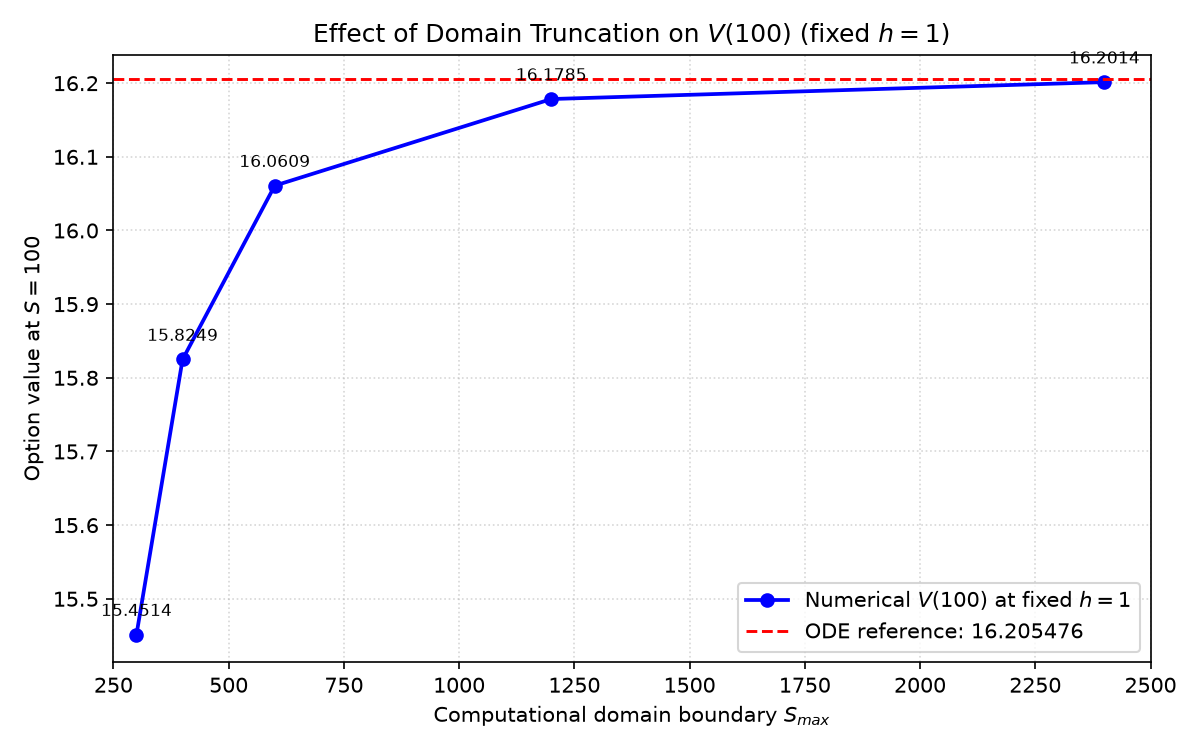
\includegraphics[width=0.92\textwidth]{smax_study.png}
\caption{Effect of domain truncation on $V(100)$ at fixed $h=1$. The value
approaches the $S_{\max}=2400$ sample from below as the domain is enlarged.
The curve approaches the independent infinite-domain reference from below;
the remaining gap at the production domain is a combination of far-field
truncation and spatial discretisation, not a pure truncation measure.}
\label{fig:smax}
\end{figure}

\subsection{Main Results}
The Delta and Gamma profiles in Figure~\ref{fig:greeks} are computed from
the local-volatility solution by finite differences on the same grid. In the
exercise region $V=K-S$, so $\Delta=-1$ and $\Gamma=0$. In the continuation
region Delta rises toward zero and Gamma becomes positive. The free boundary
is a point of $C^1$ but not $C^2$ matching: Gamma jumps across $S^*$, and the
discrete derivative localises the jump as a narrow positive peak.

\begin{figure}[H]
\centering
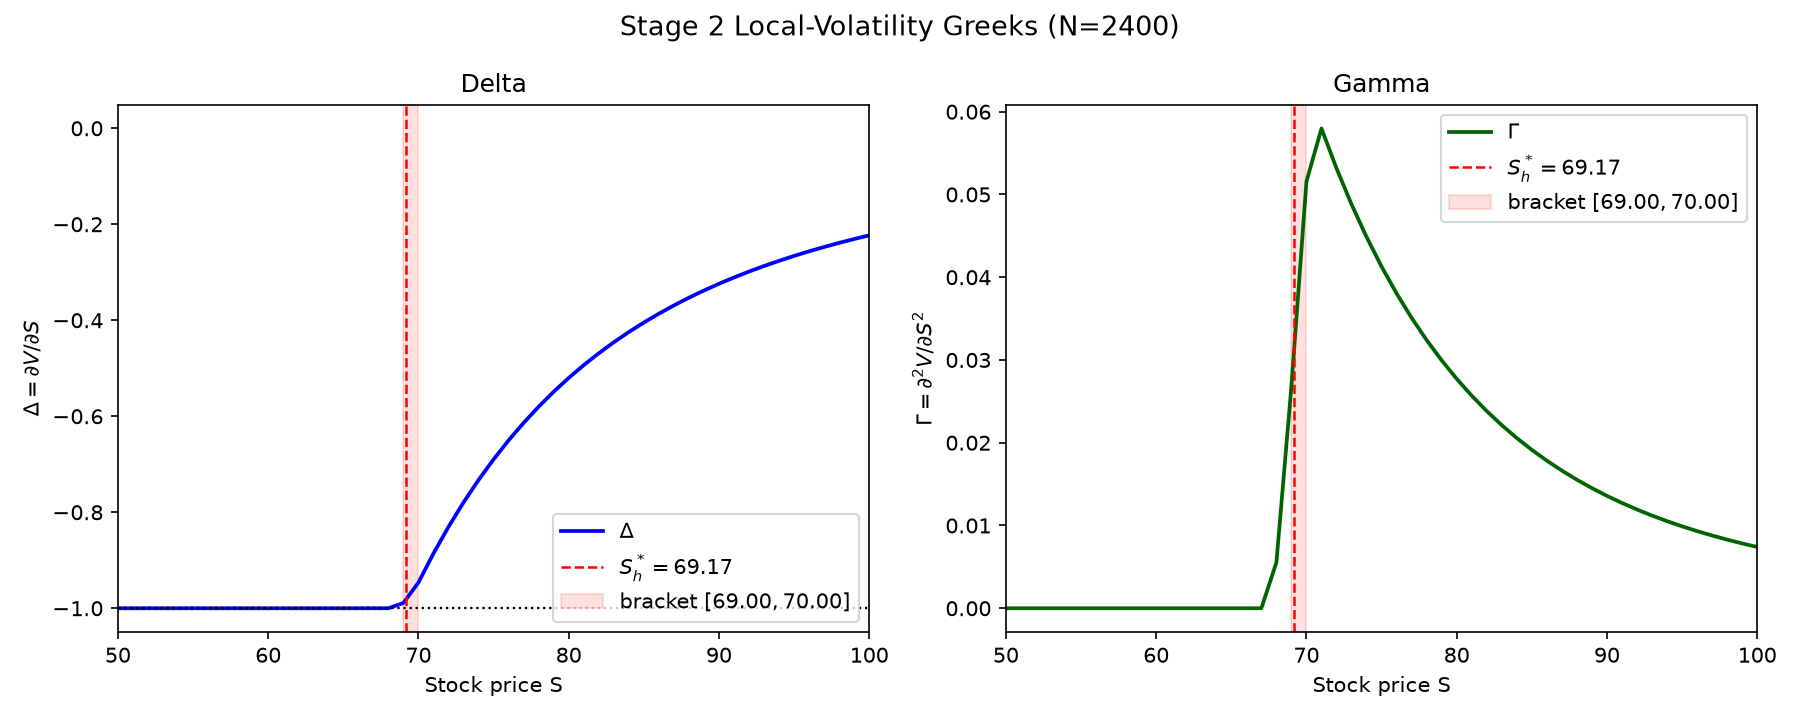
\includegraphics[width=0.98\textwidth]{greeks.png}
\caption{Stage~2 Delta and Gamma at $N=2400$. Delta is $-1$ on the exercise
side and increases toward zero in the continuation region. Gamma is zero
where the payoff is active and has a sharp positive peak near the free
boundary. The dashed line marks $S_h^*=69.17$; the shaded band is the
bracket $[69,70]$. The peak is a mesh-localised representation of the
curvature jump, not a smooth physical maximum.}
\label{fig:greeks}
\end{figure}

The peak height is therefore mesh dependent, but it does not exhibit the
$1/h$ growth of a discontinuity. The measured maxima on
$N=600,1200,2400,4800$ are $3.96\times10^{-2}$, $5.22\times10^{-2}$,
$5.80\times10^{-2}$, and $6.32\times10^{-2}$: refining $h$ by a factor of
eight increases the peak by only $1.60$. The free boundary has $C^1$ but not
$C^2$ matching, so Gamma has a jump; the finite-difference stencil spreads
that jump over adjacent cells. The sign and location of the transition are
the stable quantities, while the peak height is not a physical derivative
and should not be used for convergence.

At $S=100$ the local-volatility Delta is approximately $-0.223$, compared
with $-0.292$ for constant $\sigma=0.20$ and the same $q=0.02$. Thus its
magnitude is smaller, not larger. This is not a pointwise volatility effect:
the local-volatility profile equals $0.20$ at $S=100$ and is higher above
that price, which raises the continuation premium and reduces the put's
exercise sensitivity there.

\subsection{Adjoint Sensitivity}
\label{sec:sensitivity}
The discrete adjoint system \eqref{eq:adjoint-system}--\eqref{eq:adjoint-derivative}
is evaluated at $S=100$, $N=4800$, $S_{\max}=2400$, and the converged active
set of the benchmark. The objective is $J=V(100)$; the interpolation weights
select the corresponding grid value. For each parameter, the operator
derivatives are assembled by centred differences with step $10^{-5}$.
Table~\ref{tab:adjoint} compares the adjoint derivative with the derivative
obtained by solving the full LCP twice and with the exact analytic
derivative. The adjoint and direct finite differences agree to better than
$2\times10^{-9}$; their common difference from the analytic value is the
remaining spatial discretisation error.

\begin{table}[H]
\centering
\resizebox{\textwidth}{!}{%
\begin{tabular}{cccccc}
\toprule
\textbf{Parameter} & \textbf{Exact derivative} & \textbf{Adjoint} &
\textbf{Direct FD} & \textbf{Absolute error} & \textbf{Relative error} \\
\midrule
$\sigma$ & $1.036337\times10^{2}$ & $1.033137\times10^{2}$ &
$1.033137\times10^{2}$ &
$3.201\times10^{-1}$ & $0.309\%$ \\
 $r$ & $-2.072675\times10^{2}$ & $-2.066273\times10^{2}$ &
$-2.066273\times10^{2}$ &
$6.401\times10^{-1}$ & $0.309\%$ \\
 $q$ & $1.480482\times10^{2}$ & $1.475971\times10^{2}$ &
$1.475971\times10^{2}$ &
$4.511\times10^{-1}$ & $0.305\%$ \\
\bottomrule
\end{tabular}
}
\caption{Discrete adjoint sensitivities of $V(100)$ at $N=4800$. The adjoint
and the direct full-LCP finite differences agree to better than
$2\times10^{-9}$. The exact derivative is available only for the
constant-volatility benchmark; it isolates the common spatial error of both
numerical derivatives. The signs agree with the financial interpretation:
higher volatility and dividend yield raise the put value, while a higher
risk-free rate lowers it.}
\label{tab:adjoint}
\end{table}

The sensitivity magnitudes satisfy the expected ordering: the rate
sensitivity is about twice the volatility sensitivity because $r$ enters
both discounting and the drift, whereas $\sigma$ enters only the diffusion
coefficient. The adjoint calculation costs one additional tridiagonal solve
after the LCP, independently of the number of parameters; a direct
finite-difference estimate requires two full nonlinear solves per parameter.
This is the main practical advantage of the adjoint formulation for
calibration and risk analysis.

\subsection{Limitations and Robustness}
The first limitation is the artificial far-field boundary. The condition
$V(S_{\max})=0$ is exact only in the infinite-domain limit. The
domain-truncation study shows that the zero-Dirichlet condition is poor on
short domains. At $S_{\max}=2400$ the pure finite-domain truncation in
\(V(100)\) is $5.578\times10^{-3}$, while the combined production error at
$h=1$ is $4.055\times10^{-3}$ because spatial and truncation errors partially
cancel. Both are about $0.025$--$0.035\%$ of the option value. The exact
far-edge value is $4.833\times10^{-1}$ and is set to zero. The asymptotic
Robin closure in
Section~\ref{sec:adaptive-experiments} reduces the error in \(V(80)\) by up
to a factor of $390$ at fixed $h$, but the local-volatility production run
retains the zero-Dirichlet condition. A larger domain or an asymptotic
local-volatility closure is therefore the appropriate next step; the
current truncation error is now quantified rather than hidden inside a
fine-grid comparison.

The second limitation is the free-boundary kink. The fitted scheme is second
order in the smooth continuation region, but the maximum norm also contains
the grid-localised position of the kink; this contribution is at most first
order and need not be monotone. On the aligned validation grid the order is
clean at two; on the production grid the contact set can remain on the wrong
side of the kink until the mesh resolves it, as the coarse Stage~1 brackets
and the $N=1200$ local-volatility bracket show. The Gamma peak is a related
localisation artefact, but its measured height grows sublinearly in this
study and is not evidence of an additional $1/h$ singularity.
The clustered grid reduces the maximum value error by a factor of $2.255$ at
$N=2400$, and its four-point boundary error is $4.553\times10^{-5}$ at
$N=4800$. A fully boundary-fitted mesh or a high-order deferred-correction
scheme \cite{ref6} could remove the remaining phase sensitivity at the cost of
additional implementation complexity.

The third limitation is the semi-analytic nature of the local-volatility
reference. The infinite-domain value requires an asymptotic tail closure at
$S_{\inf}=10^5$, and the finite-domain value is a separate shooting problem;
neither is a closed-form expression. This is nevertheless an independent
check: it does not use the finite-difference grid, the LCP solver, or the
$N=9600$ reference that the earlier version used, and its constant-volatility
special case agrees with the closed form to the tolerances stated above. A
strongly varying or discontinuous volatility profile would still require
adaptive meshing or local refinement around $S^*$. The present profile is
deliberately smooth so that the M-matrix argument and the interpolation
formula remain applicable without additional regularity assumptions.

Furthermore, the numerical solution exhibits a localised loss of regularity
at the free boundary $S^*$, visible as a sharp spike in the Gamma profile.
This is qualitatively similar to a corner singularity, but the analogy is not
used quantitatively: no $O(h^{2/3})$ rate is claimed. Local grading near
$S^*$ is implemented in Section~\ref{sec:adaptive-experiments}; a fully
front-fitted transformation remains future work.

\subsection{Boundary-Row Stress Test: Zero Flux Versus Dirichlet}
\label{sec:mixed-boundary}
This experiment tests the algebraic assembly of a Neumann row; it is not a
financially admissible left boundary for the perpetual American put. At
\(S=0\) the obstacle requires \(V(0)\ge K\), while the payoff has slope
\(-1\). A zero-flux condition \(\partial_SV(0)=0\) therefore conflicts with
immediate exercise at the origin. We retain the test only to verify that the
fitted interior operator and the active-set solver remain well conditioned
when one boundary row is changed.

The condition is imposed through a ghost node at \(S_{-1}=-h\), with the
centred closure \(V_{-1}=V_1\); interpolation at the boundary then gives
\(V_0=V_1\). Eliminating \(V_0\) from the first interior row produces
\begin{equation}
    (d_1+\ell_1)V_1+u_1V_2=F_1,
    \label{eq:zero-flux-row}
\end{equation}
so the boundary treatment changes one row while leaving the fitted interior
stencil intact. The experiment uses \(N=400\), \(S_{\max}=400\), constant
volatility, and the same active-set tolerance as the Dirichlet benchmark.
Both interior calculations, summarized in Table~\ref{tab:neumann-free-boundary}
and Figure~\ref{fig:neumann-true}, return \(S_h^*=71.916\) in the bracket
\([71,72]\). The free boundary is insensitive because the active exercise
block decouples the continuation problem from the left boundary. The endpoint
is different: \(V(0)=100\) for Dirichlet and \(V(0)=99\) for the synthetic
zero-flux closure.

The endpoint result also exposes the limitation of the test. The zero-flux
solution has \(V(0)-K=-1<0\), so it violates the obstacle at \(S=0\); the
LCP constraints were enforced at interior nodes, not at this deliberately
altered endpoint. Consequently this run is not an admissible price and is
not used for any pricing, convergence, or mixed-boundary-accuracy claim. It
only shows that the fitted interior operator remains an M-matrix: the maximum
off-diagonal is \(-4.016\times10^{-2}\) and the minimum diagonal is
\(1.045\times10^{-1}\). In a genuine barrier problem, zero flux would be
applied at a barrier where the payoff/obstacle condition is compatible with
the option contract, rather than at the exercise boundary \(S=0\) of a
vanilla put.

\begin{table}[H]
\centering
\begin{tabular}{lccc}
\toprule
\textbf{Left boundary condition} & \textbf{\(V(0)\)} &
\textbf{\(V(0)-K\)} & \textbf{\(S_h^*\)} \\
\midrule
Dirichlet, \(V(0)=K\) & \(100\) & \(0\) & \(71.916\) \\
Zero-flux Neumann, \(\partial_S V(0)=0\) & \(99\) & \(-1\) & \(71.916\) \\
\bottomrule
\end{tabular}
\caption{Boundary-row stress test at \(N=400\). The zero-flux row is an
algebraic closure, not an admissible American-put boundary condition: its
endpoint value violates the obstacle by one unit. The free-boundary agreement
is therefore evidence only for the decoupling of the interior active set.}
\label{tab:neumann-free-boundary}
\end{table}

\begin{figure}[H]
\centering
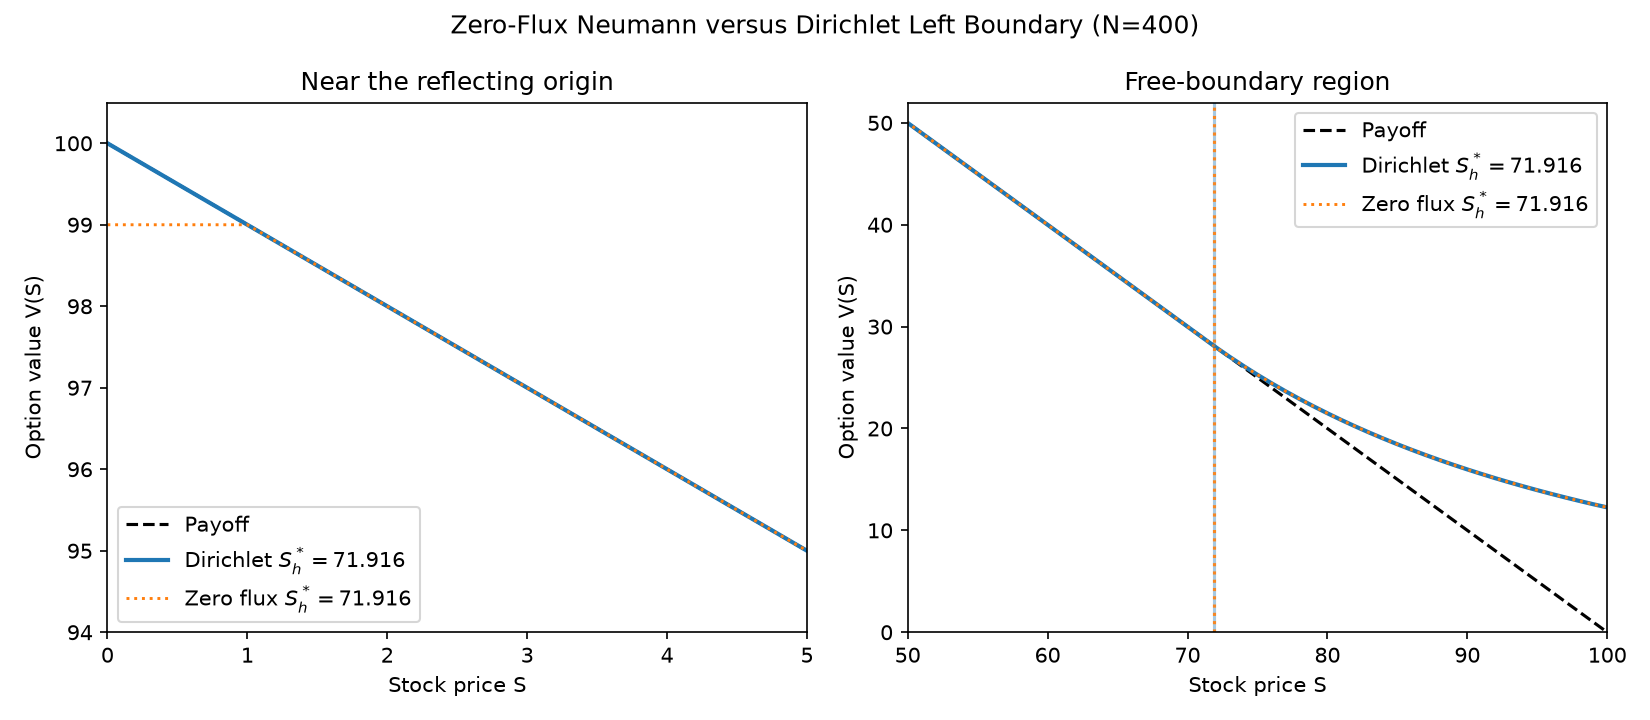
\includegraphics[width=0.9\textwidth]{neumann_true_comparison.png}
\caption{Comparison of the option value under Dirichlet and zero-flux
Neumann closures. The left panel shows the one-unit obstacle violation of the
synthetic zero-flux endpoint; the right panel shows that the interior free
boundary is unchanged.}
\label{fig:neumann-true}
\end{figure}

\subsection{2D Exploratory Extension: American Spread Put}
\label{sec:spread2d}
The preceding experiments are one-dimensional in the state variable. To test
whether the fitted M-matrix and the active-set solver survive a genuine
two-dimensional obstacle, this section adds a deliberately controlled
extension. The contract is a perpetual American spread put with payoff
\begin{equation}
    \psi(S_1,S_2)=\max(K-S_1+S_2,0).
    \label{eq:spread2d-payoff}
\end{equation}
Immediate exercise exchanges one unit of asset~1 for one unit of asset~2 plus
the strike, whenever that exchange has positive value. The model uses
$K=100$, $r=0.05$, $q_1=0$, $q_2=0.02$, $\sigma_1=\sigma_2=0.20$, and
$\rho=0$. The zero-correlation restriction is essential: it separates the
operator and keeps the local stencil five-point. It is not a claim that the
correlated spread-option problem has been solved.

For $\rho=0$, the continuation operator is
\begin{equation}
    \mathcal L_{2D}V
    =\frac12\sigma_1^2S_1^2V_{11}
    +\frac12\sigma_2^2S_2^2V_{22}
    +(r-q_1)S_1V_1+(r-q_2)S_2V_2-rV,
    \label{eq:spread2d-operator}
\end{equation}
and the obstacle problem is
\begin{equation}
    \min\{-\mathcal L_{2D}V,\;V-\psi\}=0.
    \label{eq:spread2d-lcp}
\end{equation}
The computational domain is $[0,L]^2$ with $L=300$. On $S_2=0$ the problem
reduces exactly to a one-dimensional put with parameters
$(r,q_1,\sigma_1)$, so the fitted 1D LCP supplies the Dirichlet data there.
The remaining closures are
\begin{align}
    V(0,S_2)&=K+S_2, &
    V(S_1,0)&=V_{\mathrm{1D}}(S_1), \label{eq:spread2d-boundary-a}\\
    V(S_1,L)&=\max(K-S_1+L,0), &
    V(L,S_2)&=\max(K-L+S_2,V_{\mathrm{1D}}(L)).
    \label{eq:spread2d-boundary-b}
\end{align}
The high-price edges are local truncation/exercise closures, not exact
infinite-domain boundary values. Their effect is measured rather than assumed
away in Table~\ref{tab:spread2d-domain}.

On a uniform grid with spacing $h=L/N$, let
$a_i^{(m)}=\tfrac12\sigma_m^2(S_i^{(m)})^2$ and
$b_i^{(m)}=(r-q_m)S_i^{(m)}$ for $m=1,2$. With
$\mathrm{Pe}_i^{(m)}=b_i^{(m)}h/a_i^{(m)}$ and
$B(z)=z/(e^z-1)$, the fitted directional weights are
\begin{equation}
    \ell_i^{(m)}=-\frac{a_i^{(m)}}{h^2}B(\mathrm{Pe}_i^{(m)}),
    \quad
    u_i^{(m)}=-\frac{a_i^{(m)}}{h^2}B(-\mathrm{Pe}_i^{(m)}),
    \quad
    d_i^{(m)}=\frac{a_i^{(m)}}{h^2}
    \bigl[B(\mathrm{Pe}_i^{(m)})+B(-\mathrm{Pe}_i^{(m)})\bigr].
    \label{eq:spread2d-weights}
\end{equation}
The row-ordered matrix therefore has the five entries
$\ell_i^{(1)},u_i^{(1)},\ell_j^{(2)},u_j^{(2)}$ off the diagonal and
\begin{equation}
    D_{ij}=d_i^{(1)}+d_j^{(2)}+r
    \label{eq:spread2d-diagonal}
\end{equation}
on it. Since $B(z)>0$, every off-diagonal entry is non-positive. Moreover,
$\ell_i^{(m)}+d_i^{(m)}+u_i^{(m)}=0$, so every row satisfies
\begin{equation}
    D_{ij}+\ell_i^{(1)}+u_i^{(1)}+\ell_j^{(2)}+u_j^{(2)}=r>0.
    \label{eq:spread2d-rowsum}
\end{equation}
Thus the assembled operator is strictly diagonally dominant and is an
M-matrix. A non-zero correlation would add the mixed term
$2\rho\sigma_1\sigma_2S_1S_2V_{12}$ and require a nine-point stencil; the
five-point positivity argument would no longer apply automatically.

The discrete LCP is solved by the same policy-iteration principle as in the
one-dimensional case. Active rows are replaced by identity rows with right-hand
side $\psi_{ij}$, inactive rows retain the fitted five-point stencil, and each
policy step uses one sparse direct solve. The stopping test is
$\max|\Delta V|<10^{-12}$ together with an active set that is unchanged on two
consecutive iterations. Table~\ref{tab:spread2d} reports three meshes; $N$ is
the number of intervals in each coordinate, so the finest grid has
$321\times321$ nodes and $101{,}761$ interior unknowns.

\begin{table}[H]
\centering
\scriptsize
\setlength{\tabcolsep}{4pt}
\begin{tabular}{rrrrrr}
\toprule
$N$ & \textbf{Unknowns} & \textbf{Iterations} & \textbf{Time (s)} &
\textbf{$E_{[0,200]^2}$} & \textbf{LCP residual} \\
\midrule
80  & 6{,}241   & 25 & 0.084 & $4.070\times10^{-2}$ & $6.366\times10^{-12}$ \\
160 & 25{,}281  & 50 & 0.787 & $1.611\times10^{-2}$ & $4.366\times10^{-11}$ \\
320 & 101{,}761 & 99 & 7.483 & reference            & $2.474\times10^{-10}$ \\
\bottomrule
\end{tabular}
\caption{Controlled 2D spread-put LCP with $\rho=0$. The reference is
$N=320$ on the same truncated domain, so this is a self-convergence estimate,
not an independent reference solution. $E_{[0,200]^2}$ is the maximum nodal
error against that reference in the pricing window $S_1,S_2\le200$. The
error ratio between $N=80$ and $N=160$ is $2.53$; because the grid ratio is
$2$, the implied effective order is $\log_2(2.53)=1.34$. The curved contact
set crosses the mesh, so no clean second-order rate is claimed. Times are
from one representative run and include assembly, the 1D boundary solve, and
all policy iterations.}
\label{tab:spread2d}
\end{table}

All three discretisations have minimum diagonal $1.562\times10^{-1}$,
maximum off-diagonal $0$, and minimum row sum $5.000\times10^{-2}$. The
last number is $r$, as required by \eqref{eq:spread2d-rowsum}; the M-matrix
property is therefore checked numerically as well as by construction. The LCP
residual stays below $2.5\times10^{-10}$, and the obstacle constraint is
satisfied at every node. The exercise set occupies approximately $61\%$ of the
interior grid. This fraction is diagnostic of the payoff geometry and is not
itself an accuracy indicator.

Figure~\ref{fig:spread2d} shows the value surface and the computed contact set
on the finest mesh. The exercise region is not a half-line: it is bounded by a
monotone curve $S_1=b_h(S_2)$ whose intercept at $S_2=0$ is the familiar
one-dimensional put boundary and which moves to the right as $S_2$ increases.
The black curve is the zero-slack level $V_h-\psi_h=0$. The surface is smooth
inside each region and has a value kink across that curve, as expected for an
American obstacle problem.

\begin{figure}[H]
\centering
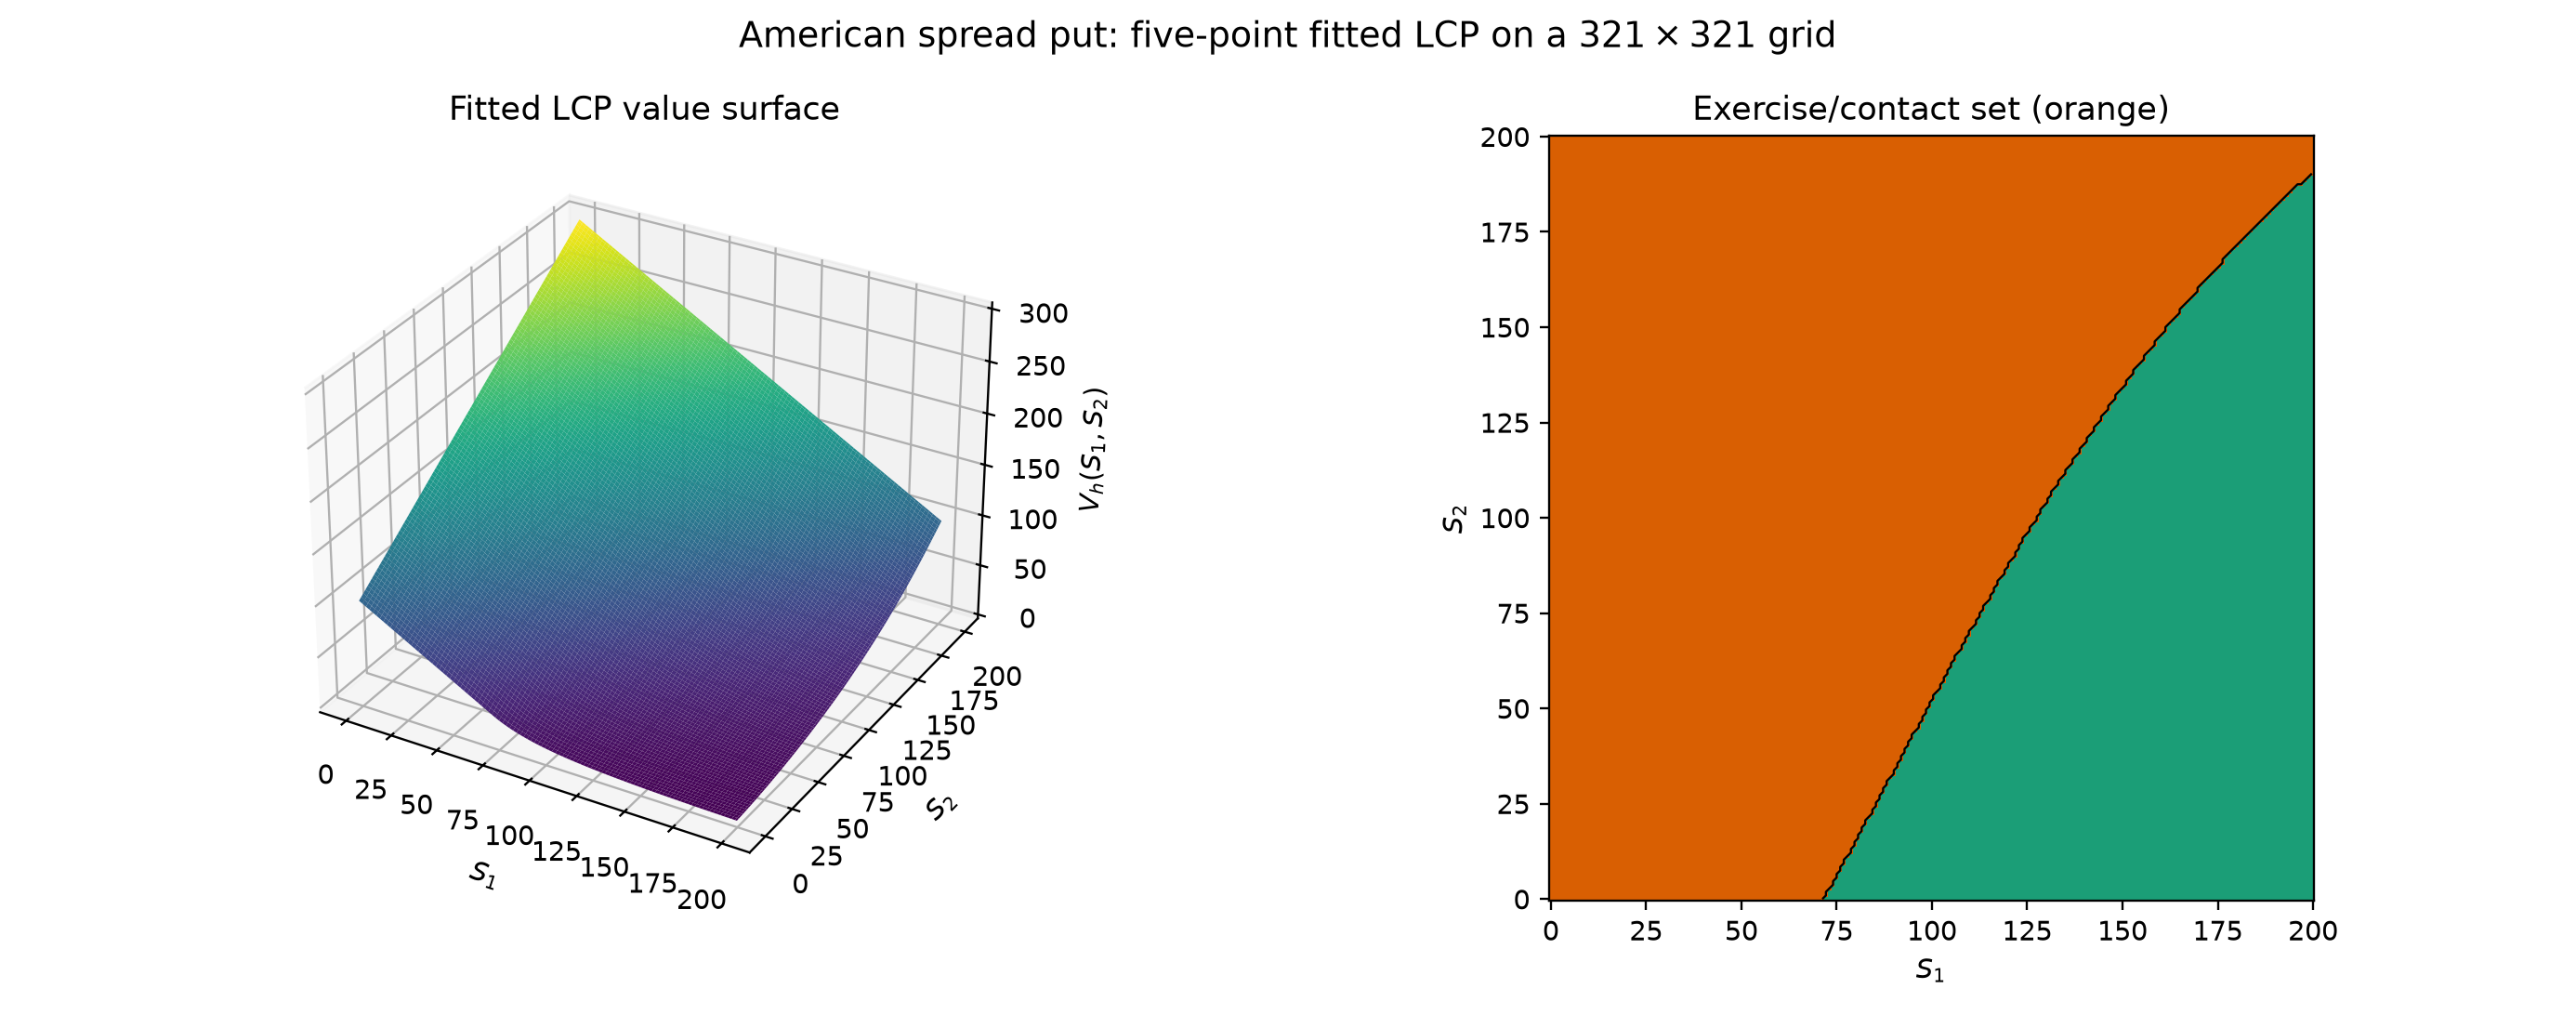
\includegraphics[width=0.98\textwidth]{spread2d_plot.png}
\caption{Controlled American spread-put LCP on the $N=320$ mesh. Left: fitted
value surface restricted to $S_1,S_2\le200$. Right: continuation region
(green), exercise region (orange), and the zero-slack contact curve (black).
The exercise boundary increases with $S_2$, so the two-dimensional contact set
is a curved region rather than a vertical or horizontal line. This matters
because it shows that the five-point fitted formulation still produces a
coherent contact set when the same active-set solver is scaled to two assets;
it is a structural test, not a production multi-asset claim.}
\label{fig:spread2d}
\end{figure}

The domain-truncation check in Table~\ref{tab:spread2d-domain} holds the mesh
fixed at $N=80$ and changes only $L$. At $(S_1,S_2)=(100,50)$, a point in the
continuation region, the $L=300$ and $L=400$ values differ by
$9.71\times10^{-4}$ (relative difference $1.9\times10^{-5}$). The shorter
domain $L=240$ differs from $L=400$ by $4.45\times10^{-2}$. This supports
$L=300$ for the reported pricing window while making the truncation explicit.
The high-price corner is more sensitive to the local payoff closure, which is
why the mesh error above is restricted to $[0,200]^2$ and why no claim of a
completed correlated two-dimensional solver is made.

\begin{table}[H]
\centering
\small
\begin{tabular}{rrr}
\toprule
$L$ & $V(100,50)$ & Difference from $L=400$ \\
\midrule
240 & 50.006716 & $-4.455\times10^{-2}$ \\
300 & 50.052234 & $9.713\times10^{-4}$ \\
400 & 50.051263 & --- \\
\bottomrule
\end{tabular}
\caption{Fixed-mesh domain-truncation check for the 2D spread put at
$N=80$. All rows use the same five-point fitted operator and high-price
closure. The $L=300$ and $L=400$ results agree well at the selected
continuation-region point, whereas the shorter domain is visibly affected by
the artificial boundary.}
\label{tab:spread2d-domain}
\end{table}

This extension demonstrates scaling rather than a full production treatment
of multi-asset options. The sparse solve reaches $10^5$ unknowns on a laptop
without changing the active-set algorithm, and the fitted five-point operator
retains the sign pattern that makes policy iteration reliable. The unresolved
parts are the correlation term and the exact far-field conditions. Both are
natural next steps: a nine-point cross-derivative stencil, a positivity
preserving treatment of $\rho\ne0$, and an asymptotic or domain-decomposition
closure for the high-price edges.

\newpage
% ============================================================
\section{Conclusions}
\label{sec:conclusions}
% ============================================================


\begin{itemize}[leftmargin=2em]
\item \textbf{Exponential Fitting and M-Matrix.} Exponential fitting produced an M-matrix at every cell Péclet number, including the degenerate region near \(S=0\). The fitted weights eliminated the central-difference oscillation without a limiter or a start-up correction, and the discrete maximum principle supplied a unique obstacle solution.

\item \textbf{Constant-Volatility Verification.} Only the production \(N=2400\) contact bracket \([71,72]\) contains the exact free boundary \(S^* = 71.4286\); at \(N=600\), \(N=1200\), and \(N=4800\) the discrete transition lies to its right. A boundary-aligned validation grid, constructed with the exact boundary, gives second-order errors with ratios \(3.990\), \(4.001\), and \(3.997\). This verifies the fitted stencil; it is not claimed as blind free-boundary recovery.

\item \textbf{Computational Efficiency.} Policy iteration required 301 iterations and 0.045 s, compared with 96,600 iterations and 20.635 s for residual-controlled PSOR. The measured wall-time ratio is \(4.6 \times 10^2\) and the iteration ratio is 321, placing the acceleration in the several-hundred-fold range. The two discrete solutions differ by \(5.685 \times 10^{-10}\), and both final LCP residuals are below \(10^{-10}\), so the algebraic error is negligible relative to the spatial and truncation errors.

\item \textbf{Local Volatility and Independent Reference.} The local-volatility experiment with \(q = 0.02\) gave \(S_h^* = 69.1688\) in the production bracket \([69.00, 70.00]\) at \(N=2400\). The coarse \(N=1200\) bracket \([70.00,72.00]\) misses the finite-domain reference \(69.1701793435\); this is disclosed as a contact-set localisation error. An independent DOP853 shooting solution gives the infinite-domain boundary \(S^* = 69.1664297389\), the finite-domain boundary \(69.1701793435\), and \(V(100)=16.2054760891\). The boundary-aligned validation errors decrease as \(3.2218\times10^{-2}\), \(8.0948\times10^{-3}\), \(2.0239\times10^{-3}\), and \(5.0610\times10^{-4}\), with observed orders \(1.993\), \(2.000\), and \(2.000\). The production errors decrease overall, but their successive ratios are \(1.21\), \(14.98\), and \(1.62\), so the sequence is not a usable refinement-rate estimate; the kink phase and coarse contact-set localisation explain the irregularity. The pure finite-domain truncation at \(S=100\) is \(5.578\times10^{-3}\), while the \(N=2400\) production total error is \(4.055\times10^{-3}\); the far-edge truncation is \(4.833\times10^{-1}\).

\item \textbf{Adaptive Mesh and Far-Field Closure.} The nonuniform fitted operator retained non-positive off-diagonals and strict diagonal dominance. With a node at the analytic boundary, clustering reduced the maximum value error by a factor of \(2.255\) at \(N=2400\); the clustered error ratios were \(3.982\), \(4.002\), and \(3.999\). The asymptotic Robin condition at \(S_{\max}=400\) reduced the error in \(V(80)\) from \(2.507\times10^{-2}\) to \(6.423\times10^{-5}\), a factor of \(390\). Both improvements reuse the same policy-iteration solver.

\item \textbf{Adjoint Sensitivities.} A single transposed sparse solve produced the sensitivities of \(V(100)\) to \(\sigma\), \(r\), and \(q\). The adjoint and direct finite differences agree to \(2\times10^{-9}\), and the relative error against the exact constant-volatility derivatives is at most \(0.31\%\). This makes parameter risk inexpensive even when the free boundary changes with the parameter.

\item \textbf{Controlled 2D Extension.} A five-point fitted LCP for an American spread put with \(\rho=0\) retained non-positive off-diagonals, a positive diagonal, and the strict row sum \(r\) on grids up to \(101{,}761\) interior unknowns. The pricing-window error decreased from \(4.070\times10^{-2}\) to \(1.611\times10^{-2}\) between \(N=80\) and \(N=160\) against an \(N=320\) self-convergence reference; the corresponding error ratio is \(2.53\) and the implied order is \(1.34\). The \(L=300\) and \(L=400\) values at \((100,50)\) differed by \(9.71\times10^{-4}\). The exercise set was a curved region whose boundary increased with \(S_2\). This experiment establishes scaling and structural robustness, not a completed multi-asset solver: the reference is not independent, and the exact high-price closure and correlated cross-derivative term remain outside its scope.

\item \textbf{Cross-directional Extensions.} Section~\ref{sec:mixed-boundary} verifies the algebraic assembly of a zero-flux row and its M-matrix structure, but the resulting endpoint \(V(0)=99\) violates the obstacle and is not an admissible American-put price. No pricing or second-order accuracy claim is made for that stress test. The controlled 2D experiment above sets \(\rho=0\) so that the five-point M-matrix proof remains valid. For \(\rho\ne0\), the free boundary is a curve and the cross-derivative term requires a nine-point stencil; a positivity-preserving treatment and compatible barrier closures remain future work.
\end{itemize}



\newpage
% ============================================================
\addcontentsline{toc}{section}{References}
\begin{thebibliography}{9}
\bibitem{ref1} J.~C.~Hull, \emph{Options, Futures, and Other Derivatives},
10th edition. Pearson, 2018.

\bibitem{ref2} P.~Wilmott, S.~Howison, and J.~Dewynne,
\emph{The Mathematics of Financial Derivatives: A Student Introduction}.
Cambridge University Press, 1995.

\bibitem{ref3} M.~Sari and S.~Gulen, Valuation of the American put option
as a free boundary problem through a high-order difference scheme.
\emph{International Journal of Nonlinear Sciences and Numerical
Simulation}, 23(7--8):1001--1015, 2021.

\bibitem{ref4} D.~L.~Scharfetter and H.~K.~Gummel, Large-signal analysis of
a silicon Read diode oscillator. \emph{IEEE Transactions on Electron
Devices}, 16(1):64--77, 1969.

\bibitem{ref5} P.~Virtanen et al., SciPy 1.0: fundamental algorithms for
scientific computing in Python. \emph{Nature Methods}, 17:261--272, 2020.

\bibitem{ref6} D.~Wang, K.~Serkh, and C.~Christara, A high-order deferred
correction method for the solution of free boundary problems using penalty
iteration, with an application to American option pricing.
\emph{Journal of Computational and Applied Mathematics},
432:115272, 2023.

\bibitem{ref7} R.~A.~Howard, \emph{Dynamic Programming and Markov
Processes}. MIT Press, 1960.

\bibitem{ref8} L.~B.~G.~Andersen and R.~Brotherton-Ratcliffe, The equity
option volatility smile: an implicit finite-difference approach.
\emph{The Journal of Computational Finance}, 1(2):5--37, 1997.

\bibitem{ref9} D.~K.~Yadav, A.~Bhardwaj, and A.~Kumar, Operator splitting
method to solve the linear complementarity problem for pricing American
option: an approximation of error. \emph{Computational Economics},
64(6):3353--3379, 2024.
\end{thebibliography}

\newpage
% ============================================================
\appendix
\section{AI Transparency Log}
\label{app:ai}
% ============================================================

The AI record below covers the project conversation with OpenAI Codex during
2--8 November 2026. AI output was treated as a proposal. Yijian Huang also
performed an independent code and experiment audit, recorded in
\texttt{AUDIT\_REPORT.md}; that audit, rather than the AI text itself, is the
main evidence for the decisions below.

\subsection*{A1. AI tools used}
\begin{table}[H]
\centering
\small
\begin{tabular}{@{}p{3.2cm}p{4.4cm}p{6.4cm}@{}}
\toprule
\textbf{Tool} & \textbf{Version / date} & \textbf{Primary use} \\
\midrule
OpenAI Codex & Project conversation, 2--8 Nov 2026 &
Mathematical checking, debugging code, drafting plotting utilities, diagnosing
irregular convergence ratios, and editing report prose. Routine LaTeX
formatting and spelling corrections are summarised by this entry rather than
logged separately. \\
\bottomrule
\end{tabular}
\end{table}

\subsection*{A2. Significant AI-assisted claim audits}
\begin{table}[H]
\centering
\scriptsize
\setlength{\tabcolsep}{4pt}
\begin{tabular}{@{}p{0.04\textwidth}p{0.43\textwidth}p{0.45\textwidth}@{}}
\toprule
\textbf{No.} & \textbf{Prompt / claim / assumptions} & \textbf{Risk and possible falsifier} \\
\midrule
1 & \textbf{Figure generation and irregular ratios.} The conversation asked
why the observed ratios changed from mesh to mesh and how the figures were
generated. The proposed explanation assumed that the free-boundary kink, the
far-field boundary and the grid phase could dominate a raw production norm. &
A convincing explanation could hide a wrong stencil or a stale figure. A
boundary-aligned grid should recover an order near two, and regenerating from
the experiment code should change every figure that previously used a literal
array. \\
2 & \textbf{Stage~2 problem definition.} The requested correction was
$q=0.02$ with the production condition $V(S_{\max})=0$, and a bracketed rather
than snapped free boundary. The assumption was that an early run had solved a
different problem and had used the analytic tail as a boundary value. &
The code could solve the wrong dividend problem or silently impose the answer.
A falsifier is disagreement with the independent DOP853 reference or with a
fixed-$h$ $S_{\max}$ sweep. \\
3 & \textbf{Fitted stencil and computed figures.} The proposed change was to
use exponential fitting and to replace literal plotting arrays by calls to the
experiment functions. The assumption was that the fitted weights preserve the
M-matrix sign pattern at every cell P\'eclet number. &
The solve could look stable while the assembled matrix has positive
off-diagonals, or a figure could remain stale. A falsifier is a positive
assembled off-diagonal, failure of the negative control, or a figure that does
not change when the experiment is rerun. \\
\bottomrule
\end{tabular}
\end{table}

\subsection*{A3. Independent verification and decision}
\begin{table}[H]
\centering
\scriptsize
\setlength{\tabcolsep}{4pt}
\begin{tabular}{@{}p{0.04\textwidth}p{0.46\textwidth}p{0.42\textwidth}@{}}
\toprule
\textbf{No.} & \textbf{Independent check and evidence location} & \textbf{Decision / modification / limitation} \\
\midrule
1 & Yijian Huang's audit (\texttt{AUDIT\_REPORT.md}, findings F5 and F12)
identified the one-sided free-boundary snap and the misleading raw-grid order.
The audit was rerun independently, and the aligned sequence was rebuilt in
\texttt{grids.py} and \texttt{experiment\_convergence.py}. & The production
bracket and a boundary-aligned order study are now reported separately.
Limitation: the production contact bracket still depends on the kink phase. \\
2 & The exact closed form \eqref{eq:exactvalue}--\eqref{eq:exactboundary} and
the independent DOP853 solver in \texttt{reference\_solution.py} were used as
oracles. \texttt{stage2\_convergence\_report.py} reproduced the mesh sequence,
and the fixed-$h$ study isolated truncation in Table~\ref{tab:smax}. &
\texttt{stage2\_local\_volatility.py} now uses $q=0.02$ and
$V(S_{\max})=0$; LCP diagnostics were added and the Stage~2 results were
regenerated. Limitation: the comparison is finite-domain and the local-volatility
reference is semi-analytic rather than closed form. \\
3 & \texttt{plot\_matrix\_spy.py} and \texttt{experiment\_central\_diff.py}
were used to inspect the assembled sign pattern and the negative control.
The audit finding F8 showed that the earlier backward-difference stencil
required a non-consistent limiter. \texttt{plot\_solver\_comparison.py},
\texttt{plot\_smax\_study.py} and \texttt{plot\_greeks.py} were changed to use
computed results rather than literal arrays. & The production assembly now
uses fitted weights in \texttt{stage1\_validation.py}; the M-matrix assertion
and residual checks remain active. Limitation: the two-dimensional extension
is restricted to $\rho=0$ and approximate high-price closures. \\
\bottomrule
\end{tabular}
\end{table}

\subsection*{A4. Intellectual ownership declaration}
Each member affirms below that they can explain and modify the listed
team-owned code, justify the mathematical claims, and describe the assumptions
and tests at the library interface without AI assistance during the viva.
\begin{table}[H]
\centering
\scriptsize
\setlength{\tabcolsep}{4pt}
\begin{tabular}{@{}p{2.1cm}p{2.5cm}p{5.2cm}p{4.1cm}@{}}
\toprule
\textbf{Name} & \textbf{Signature / date} & \textbf{Team-owned artefact / contribution} &
\textbf{Trusted dependency and interface} \\
\midrule
Yuhan Cheng & \textit{Yuhan Cheng}, 8 Nov 2026 &
Fitted operator and LCP solver, free-boundary rule, convergence and truncation
experiments, figures, tolerance sweep, and manuscript integration. &
NumPy arrays; SciPy \texttt{diags} and \texttt{spsolve}; Matplotlib output.
Checked by the M-matrix assertion, exact benchmark, and residual tests. \\
Yijian Huang & \textit{Yijian Huang}, 8 Nov 2026 &
Independent code/experiment audit, Stage~1--2 verification, reference-solver
cross-checks, plotting and result validation. &
SciPy DOP853 \texttt{solve\_ivp}, CSV outputs, and the closed-form benchmark.
The interface was checked against the exact constant-volatility solution. \\
\bottomrule
\end{tabular}
\end{table}

\newpage
% ============================================================
\section{Individual Contribution Statements}
\label{app:ics}
% ============================================================

The project had two members. Each statement below is specific to that member
and lists files or sections that can be checked in the repository.

\subsection*{ICS 1 --- Yuhan Cheng (Student ID: 2685836)}
\begin{formbox}
\small
\textbf{Role:} Algorithm Implementation, Mathematical Theory, Visualisation,
and Report Writing.

\textbf{1. Specific contributions to this project:}
\begin{itemize}[leftmargin=1.4em, itemsep=1pt]
\item Derived and implemented the fitted Scharfetter--Gummel operator, the
policy-iteration LCP solver, residual and shape diagnostics, and the
free-boundary bracket in \path{stage1_validation.py}.
\item Built the aligned and production convergence experiments in
\path{grids.py}.\newline
\path{experiment_convergence.py} regenerates the aligned table.
\item Implemented the Stage~2 local-volatility solve and four-mesh study in
\newline\path{stage2_local_volatility.py} and
\path{stage2_convergence_report.py}.
\item Implemented the adaptive-grid, Robin-closure and adjoint extensions in
\path{advanced_methods.py}, the 2D spread-put experiment in
\path{stage2d_spread.py}, and the solver/tolerance sweep in
\path{experiment_solvers.py}. I also wrote the plotting scripts and
integrated the figures and text into the report.
\end{itemize}

\textbf{2. Hardest conceptual obstacle encountered and how it was addressed:}
My first instinct was that an irregular refinement ratio meant the stencil or
solver was wrong. The audit showed three competing effects: the free-boundary
kink changes phase with the mesh, the finite-domain tail is not zero, and the
active-set estimate is only first-order in the boundary location. I separated
a boundary-aligned validation sequence from the production contact bracket,
compared the fitted solve with the closed form and DOP853 reference, and
reported the truncation study at fixed $h$ instead of tuning the code to a
desired ratio.

\textbf{3. One AI-generated output used, and what was changed:}
In the Codex conversation I asked why the ratios were irregular and how to
regenerate the figures. The AI suggested explanations and plotting changes,
but I did not treat the explanation as evidence. I changed the experiments to
use boundary-aligned grids, separated the kink and truncation effects,
replaced literal plotting arrays with computed results, regenerated the
figures, and checked the changes against Yijian Huang's audit (A2--A3).

\textbf{4. One point still not fully understood:}
I do not yet have a sharp-interface proof of the exact convergence rate of the
discrete free boundary; the report therefore claims a bracket and a
second-order aligned value error, not a second-order boundary-recovery rate.
The conditioning of the direct solve is also checked empirically rather than
bounded analytically.

\textbf{Signature:} \textit{Yuhan Cheng} \quad
\textbf{Date:} 8 November 2026
\end{formbox}

\newpage
\subsection*{ICS 2 --- Yijian Huang (Student ID: 2685589)}
\begin{formbox}
\small
\textbf{Role:} Project Manager, Testing and Verification.

\textbf{1. Specific contributions to this project:}
\begin{itemize}[leftmargin=1.4em, itemsep=1pt]
\item Read the solver, Stage~2 wrapper, experiment drivers and plotting code,
ran the scripts independently, and recorded the findings in
\texttt{AUDIT\_REPORT.md}. I checked the LCP formulation, residuals, obstacle
constraints, monotonicity, convexity, contact-set structure, and the reported
free-boundary rules.
\item Cross-checked the Stage~1 results against the closed-form values and the
Stage~2 results against \texttt{reference\_solution.py} (DOP853 shooting). I
reviewed the fixed-$h$ truncation study, the four-mesh convergence tables, the
2D spread-put checks, and the final tolerance sweep.
\item The audit identified the Stage~2 $q=0$ error, the analytic boundary that
supplied the answer, the depth-changing $S_{\max}$ study, the snapped free
boundary and literal plotting arrays. After the fixes I verified that
\path{stage1_validation.py}, \path{stage2_local_volatility.py},
\path{experiment_convergence.py}, \path{stage2_convergence_report.py},
\path{experiment_solvers.py}, and the plotting scripts produced the
reported data on rerun.
\end{itemize}

\textbf{2. Hardest conceptual obstacle encountered and how it was addressed:}
The hardest part was distinguishing a genuine numerical defect from a visual
or mesh artefact. A smooth-looking figure can still be stale, and a poor
refinement ratio can come from the moving free-boundary kink, the truncated
domain, or the algebraic solve. I used independent oracles and controlled
experiments: the exact solution, DOP853, fixed-$h$ domain sweeps, matched
solvers, and a residual tolerance sweep. This made each claimed error source
testable rather than a matter of appearance.

\textbf{3. One AI-generated output used, and what was changed:}
I used the same Codex conversation to organize audit hypotheses and trace
suggested code changes. I accepted a claim only after reading the relevant
implementation and reproducing it with the project scripts. The audit findings
led to changes in the Stage~2 dividend and boundary setup, the free-boundary
bracket and diagnostics, the plotting scripts, the fitted-stencil assembly,
and the tolerance evidence retained in this report (A2--A3).

\textbf{4. One point still not fully understood:}
The sharp convergence rate of the free boundary for a nonsmooth payoff and the
extension of the positivity-preserving proof to correlated two-asset problems
remain open. The current two-dimensional test is therefore limited to
$\rho=0$ and is not presented as a production multi-asset solver.

\textbf{Signature:} \textit{Yijian Huang} \quad
\textbf{Date:} 8 November 2026
\end{formbox}

\newpage
% ============================================================
\section{Supplementary Figures and Data}
\label{app:validation}
% ============================================================

All numerical experiments, figures, and diagnostic checks reported in this
work are reproducible from a single command in the project directory:
\texttt{python run\_all.py}. The orchestrator executes the solver and
experiment scripts in dependency order, regenerates every figure and
\texttt{stage1\_convergence.csv}, \texttt{stage2\_convergence.csv},
\texttt{adaptive\_convergence.csv}, \texttt{tolerance\_sweep.csv},
\texttt{spread2d\_results.csv}, and \texttt{spread2d\_domain.csv}, and
terminates with an error if any required artifact is missing.

\begingroup
\setlength{\tabcolsep}{4pt}
\renewcommand{\arraystretch}{1.08}
\setlength{\LTpre}{0.25cm}
\setlength{\LTpost}{0.15cm}
\begin{longtable}{@{}p{0.16\textwidth}p{0.28\textwidth}p{0.18\textwidth}p{0.16\textwidth}p{0.08\textwidth}@{}}
\caption{Detailed validation criteria and pass standards for the financial
LCP solver. $^{\dagger}$The passing production-boundary checks apply to the
stated meshes; coarse contact brackets that miss $S^*$ are reported as
diagnostics in Tables~\ref{tab:stage1-production} and
\ref{tab:stage2-convergence}. ``ALG.'' denotes an algebraic stress test with
no pricing claim.}
\label{tab:validation-criteria}\\
\toprule
{\scriptsize\textbf{Check}} & {\scriptsize\textbf{What it verifies}} &
{\scriptsize\textbf{Metric}} & {\scriptsize\textbf{Pass criterion}} &
{\scriptsize\textbf{Status}} \\
\midrule
\endfirsthead
\multicolumn{5}{@{}l}{\textit{Table~\thetable\ (continued)}}\\
\toprule
{\scriptsize\textbf{Check}} & {\scriptsize\textbf{What it verifies}} &
{\scriptsize\textbf{Metric}} & {\scriptsize\textbf{Pass criterion}} &
{\scriptsize\textbf{Status}} \\
\midrule
\endhead
\bottomrule
\endfoot
\bottomrule
\endlastfoot
\scriptsize
M-matrix off-diagonals & Verifies that the discrete operator preserves the
maximum principle. & max off-diagonal & \(\le 0\) & PASS \\
M-matrix diagonals & Verifies strict diagonal dominance. & min diagonal &
\(>0\) & PASS \\
LCP complementarity & Verifies obstacle slackness and differential residual
on both stages. & \(\|\min(a_h,b_h)\|_\infty\) & \(<10^{-9}\) & PASS \\
Free-boundary bracket & Verifies the width of the bracketed free boundary.
& \(S_{\mathrm{hi}}-S_{\mathrm{lo}}\) & \(\le h\) & PASS \\
Monotonicity & Verifies the put option value is strictly decreasing.
& Boolean check & True & PASS \\
Convexity & Verifies the put option value is convex in \(S\).
& Boolean check & True & PASS \\
Value bounds & Verifies the solution stays within obstacle bounds.
& \(\psi_h\le V_h\le K\) & True & PASS \\
Solver acceleration & Verifies the iteration ratio between Policy Iteration
and PSOR. & Wall-time ratio & \(>10^2\) & PASS \\
Truncation convergence & Verifies that \(V(100)\) approaches the
infinite-domain reference as \(S_{\max}\to2400\). & Error in \(V(100)\) &
\(<10^{-2}\) & PASS \\
Stage~1 closed-form agreement & Verifies the fitted solve against the
analytic benchmark. & Aligned \(E_{4800}\) & \(<10^{-3}\) & PASS \\
Stage~1 aligned refinement & Verifies that the aligned validation bracket
contains the exact boundary and that the order is two. & Aligned bracket;
aligned error ratio & contains \(S^*\); ratio near \(4\) & PASS \\
Stage~1 production boundary & Verifies the disclosed production-boundary
error at the finest mesh. & \(|S_h^*-S^*|\) at \(N=4800\) & \(<10^{-1}\) &
PASS$^{\dagger}$ \\
Stage~2 four-mesh convergence & Verifies local-volatility discretisation
against the independent ODE reference. & Aligned \(E_{4800}\) & \(<10^{-3}\) &
PASS \\
Stage~2 production boundary & Verifies the \(N=2400\) production boundary
estimate against the finite-domain shooting boundary. &
\(|S_h^*(2400)-S_{\mathrm{finite}}^*|\) & \(<0.01\) & PASS$^{\dagger}$ \\
Stage~2 far-field truncation & Verifies that truncation is quantified
against the infinite-domain value. & Pure truncation in \(V(100)\) &
\(<10^{-2}\) & PASS \\
Contact-set structure & Verifies that the exercise region is one interval.
& Single contiguous set & True & PASS \\
Algebraic error separation & Verifies the tolerance plateau on \(N=400\)
against the direct policy-iteration reference. & \(\max|\Delta V|\);
\(|\Delta V(100)|\) at \(10^{-10}\) & \(<10^{-9}\); plateau & PASS \\
Dirichlet endpoint & Verifies the admissible American-put boundary value.
& \(|V(0)-K|\) & \(=0\) & PASS \\
Zero-flux row stress test & Verifies the altered row algebra only; the
endpoint is not an admissible price. & \(V(0)-K\) & \(-1\), documented &
ALG. \\
2D M-matrix & Verifies the five-point spread-put operator has non-positive
off-diagonals, positive diagonal, and strict row sum. & max off-diagonal;
min diagonal; min row sum & \(\le0;\ >0;\ >0\) & PASS \\
2D complementarity & Verifies the spread-put LCP on all three meshes.
& \(\|\min(a_h,b_h)\|_\infty\) & \(<10^{-9}\) & PASS \\
2D refinement and truncation & Verifies decreasing mesh error and a stable
\(L=300\) pricing window. & \(E_{160}<E_{80}\);
\(|V_{300}(100,50)-V_{400}(100,50)|\) & \(<10^{-3}\) & PASS \\
\end{longtable}
\endgroup

\noindent The machine-readable evidence is stored in the project
directory, and the complete run is regenerated via
\texttt{python run\_all.py}.

\end{document}
